\chapter{Erstellung der Computerspielengines}
\label{chapter:erstellung-der-computerspielengines}

Nachdem Patchwork auf unterschiedlichste Aspekte analysiert und das Brettspiel als Computerprogramm umgesetzt wurde, werden nachfolgend die verschiedenen Computerspielengines für das Spiel implementiert.

\section{Ansatz A: Zufallsauswahl der Spielzüge}
\label{section:erstellung-ansatz-a}

Um eine Computerspielengine zu erstellen, muss das Trait \code{Player}, welcher in Codeausschnitt \ref{code:player-trait} zu sehen ist, von der Engine implementiert werden. Dafür müssen die zwei Methoden \code{name()} und \code{get\_action()}. Die erste Methode gibt den Namen der Computerspielengine zurück, um sie während des Spiels identifizieren zu können, während die zweite Methode die Aktion als \code{PlayerResult<Action>} zurückgibt, die der Spieler machen möchte und benötigt als Eingabe den aktuellen Zustand des Spiels.

\lstinputlisting[
    label={code:player-trait},
    caption={Definition des Player-Traits},
    captionpos=b,
    language=Rust,
    firstline=0,
]{res/code/player-trait.rs}

Die einfachste Computerspielengine ist der \code{RandomPlayer}, in Codeauschnitt \ref{code:random-player} zu sehen, welcher einen Spieler repräsentiert, der zufällige Züge macht. Zur Auswahl der Züge verwendet die Engine den Zufallsgenerator Xoshiro256++, der einen der möglichen Spielzüge im aktuellen Spielzustand \code{game} auswählt, die durch den Aufruf der Methode \code{game.get\_valid\_actions()} bereitgestellt werden. Diese Computergegner ist gut für Vergleichszwecke im späteren Kapitel \nameref{chapter:evaluation} geeignet, da die zufälligen Züge eine Baseline gegen die komplexeren, strategischen Entscheidungen der anderen Computerspielengines bildet.

\lstinputlisting[
    label={code:random-player},
    caption={Definition des RandomPlayers},
    captionpos=b,
    language=Rust,
    firstline=0,
]{res/code/random-player.rs}

\pagebreak

\section{Ansatz B: Greedy-Algorithmus}

Die Computerspielengine, welche mit dem Greedy-Algorithmus arbeitet, ist ebenfalls ein weiterer guter Vergleichskandidat für die komplexeren Computergegner. Wenn der Greedy-Algorithmus vor eine Entscheidung gestellt wird, wählt dieser immer den Spielzug, der in der aktuellen Situation optimal erscheint, auch wenn der Spielzug sich im weiteren Spielverlauf nicht als bester Zug herausstellt \cite[S. 234]{2023Greedy}. Durch die direkte Bewertung mittels des Evaluators mit 1-Zug-Voraussicht ist dieses zukünftige Wissen allerdings nicht bekannt. Als einer der Evaluatoren wurde für diesen Computergegner eine \enquote{Handcrafted Evaluation} implementiert, dieser Evaluator zeichnet sich dadurch aus, dass er zahlreiche Heuristiken und Regeln verwendet, um eine Evaluierung einer Position zu determinieren \cite{2023.StockfishTerminology}. Um einen Evaluator zu erstellen, muss der Trait \code{Evaluator} implementiert werden. Dieser ist in Codeausschnitt \ref{code:evaluator} zu sehen und beinhaltet drei Methoden. Tatsächlich muss jedoch nur die erste Methode \code{evaluate\_intermediate\_node()} implementiert werden, da die anderen beiden Methoden \code{evalute\_terminal\_node()} und \code{evaluate\_node()} allgemeingültige Standardimplementierungen besitzen. Die Methoden funktionieren alle gleich: Sie nehmen den aktuellen Spielzustand an und geben dann eine Zahl aus, welche die Evaluierung der Position beschreibt, wobei eine große Zahl in negative oder positive Richtung für den jeweiligen Spieler gut ist.

\lstinputlisting[
    label={code:evaluator},
    caption={Evaluierer für den Spielzustand},
    captionpos=b,
    language=Rust,
    firstline=0,
]{res/code/evaluator.rs}

Der \enquote{Handcrafted Evaluator}, im Quellcode als \code{StaticEvaluator} bezeichnet, für diese Computerspielengine, berechnet wie folgt den Score für die aktuelle Spielposition. Es werden die Scores für beide Spieler berechnet und anschließend der ist Evaluation der Score des Spielers abgezogen vom Score des Gegners. Innerhalb der Berechnung des Scores für einen Spieler werden folgende Berechnungsgrundlagen angewandt:

Als erster Faktor wird die Spielposition, die mit den normalen Endregeln berechnet wird, als $es$ eingerechnet. Die normalen Endregeln bedeuten in diesem Fall, dass für jedes freie Feld zwei Punkte abgezogen werden und jeder Knopf, der dem Spieler gehört, mit einem Punkt gewertet wird.

Als zweiter Faktor wird mit $ps$ einberechnet, an welcher Stelle der Zeitstein des Spielers liegt. Für jedes Feld, über das der Zeitstein noch nicht gezogen ist, wird dieser Faktor mit einem Punkt mehr gewertet.

Als dritter Faktor wird die Bewertung des Ablageplans des Spielers $bs$ miteingerechnet. Dazu wird zuerst die Feldanzahl mit neun multipliziert, um immer für $bs$ eine positive Punktzahl zu bekommen. Im Fall von Patchwork mit seinen 81 Felder pro Ablageplan ist somit die intitale Punktezahl 719. Nun wird für jedes freie Feld auf dem Ablageplan neun Punkte von der Punktzahl abgezogen, somit kommt man bei einem komplett leeren Ablageplan auf einen $bs$ von null. Anschließend wird für jedes Feld, auf dem ein Teil von einem Flicken liegt, berechnet wie viele leere Nachbarfelder dieses hat und für jedes leere Feld ein Punkt abgezogen. Der Rand gilt bei dieser Berechnung als befülltes Feld, wenn er als Nachbarfeld in Frage kommt, für den Rand werden jedoch nicht die leeren Nachbarfelder bestimmt. Zur Bestimmung, was die Nachbarn eines Feldes sind, gibt es zwei klassische Nachbarschaften: Die von Neumann Nachbarschaft, wobei alle Felder als Nachbar gelten, welche eine Manhattan-Distanz entfernt sind und die Moore Nachbarschaft, bei der alle Felder als Nachbar gelten, die eine Tschebyschow-Distanz entfernt sind \cite[S. 2]{2016.kneighborhood}. In der Abbildung \ref{fig:nachbarschaften} sind diese beiden Nachbarschaften grafisch dargestellt und jeweils mit zwei Beispielen im Patchwork-Kontext versehen.

Für die Implementierung der Nachbarschaft wurde sich für die Moore Nachbarschaft entschieden, um alle umliegenden Felder des betrachten Feld abzudecken.

\begin{figure}[!ht]
    \centering
    \includegraphics[width=\textwidth]{res/pictures/nachbarschaften.pdf}
    \caption{Mögliche Nachbarschaften für den Evaluator}
    \label{fig:nachbarschaften}
\end{figure}

Als vierter Faktor wird der Knopfeinkommen-Score $bis$ miteingerechnet. Die Formel \ref{eqn:button-income-score} zur Berechnung dieses Scores benötigt die Argumente $tp$ und $bi$, wobei das erste Argument die Anzahl der schon überschrittenen Knopfwertungen beschreibt und das zweite Argument die Höhe des Knopfeinkommen vom Spieler beschreibt, also wie viele Knöpfe dieser bei Überschreiten einer Knopfwertung erhält. Je weniger Knopfwertungen vor dem Zeitstein des Spielers sind, desto weniger Nutzen besitzt eine hohes Knopfeinkommen. Daher bewertet dieser Score die untenstehende Formel mit exponentiellem Zerfall. Wurde noch keine Knopfeinkommen überschritten, so bringt jeder Knopf des Knopfeinkommes acht Punkte, wohingegen nur noch ein Punkt pro Knopf im Knopfeinkommen gewertet wird, wenn noch ein Knopfwertung aussteht.

\begin{equation}
    \label{eqn:button-income-score}
    bis(tp, bi) = 8 \cdot e^{\frac{tp}{8}\ln\left(\frac{1}{8}\right)} \cdot bi
\end{equation}

\pagebreak

Um die Evaluation für eine Spielposition zu erhalten, werden mit der folgenden Formel \ref{eqn:evaluator-score} alle Faktoren zusammengerechnet. $\tau$ beschriebt hierbei als Prozentzahl, wie weit das Spiel der Spielposition schon fortgeschritten ist. Daraus lässt sich schließen, dass zu Beginn eines Spiels der Ablageplan-Score $bs$ im Verhältnis zum Endscore $es$ viel höher gewichtet wird, um anstatt irgendwie viele Felder mit Flicken zu befüllen, die Flicken sinnvoll platziert werden, zum Beispiel am Rand oder nahtlos anschließend an andere Flicken. Beide Faktoren werden zweifachgewichtet in die Evaluation mit einberechnet, während der Positions-Score für den Zeitstein $ps$ und der Knopfeinkommen-Score $bis$ nur einfach gewichtet sind. Diese Gewichtung wurde vorgenommen, um möglichst viele Strafpunkte pro freiem Feld auf dem Ablageplans zu vermeiden und in beide vorderen Scores der Ablageplan von großer Bedeutung ist.

\begin{equation}
    \label{eqn:evaluator-score}
    eval = 2 \cdot bs \cdot (1 - \tau) + 2 \cdot es \cdot \tau + ps + bis
\end{equation}

Neben dem \enquote{Handcrafted Evaluator} gibt es noch weitere Evaluatoren, von denen zwei an dieser Stelle beschrieben werden sollen. Der Win-Loss-Evaluator lässt zur Bewertung einer Spielposition das Spiel von dieser Stelle aus zufällig zu Ende spielen und gibt dann eine 1 zurück, wenn der Spieler gewonnen hat und eine -1, wenn der Gegner in dem zufälligen Spielende gewonnen hat. Der Score-Evaluator funktioniert nach dem gleichen Prinzip des zufälligen zu Ende Spielens der Spielposition, mit dem einzigen Unterschied, dass nicht -1 oder 1 zurückgegeben wird, sondern die Differenz der Endwertung der beiden Spieler.

\pagebreak

\section{Ansatz C: Principal-Variation-Search}
\label{section:erstellung-ansatz-b}

Der dritte und erste richtige Versuch eines starken Computerspielgegners ist der \acl{PVS} Spieler. Für das Finden der besten Aktion verwenden der \acs{PVS} Spieler verwendet dabei eine optimierte Variante des Alpha-Beta-Suchalgorithmus, die \acf{PVS}. Bei der \ac{PVS} werden mehrere Änderungen vorgenommen. Zuerst wird der klassische Minimax-Algorithmus mittels Negamax implementiert. Bei Nullsummenspielen wie Patchwork ist der maximale Wert des einen Spielers immer der negierte minimale Wert des anderen Spielers ($\max\left(a,b\right) = -\min\left(-a,-b\right)$) \cite[S. 9]{2020.MinimaxTheorem}. Bei Negamax wird dies ausgenutzt, indem immer dieselbe Funktion aufgerufen wird und das Ergebnis negiert wird, anstatt zwei verschiedene Fälle für den min- und max-Spieler zu haben. Dies funktioniert aber nur, wenn der aktive Spieler nach jedem Spielzug wechselt. Dies ist in Patchwork nicht der Fall, kann in der Computerspielimplementierung aber erzwungen werden, indem der \code{do\_action} Methode ein \enquote{force player switch} Parameter übergeben wird. Würde der Spieler im Normalfall nicht wechseln, so wird einfach ein Spielerwechsel erzwungen und dem neuen Spieler nur die \emph{Phantom}-Aktion zur Verfügung gestellt. So kann auch die Suche in Patchwork ohne Probleme als Negamax implementiert werden, was die Implementierung vereinfacht. Bei Mimimax-basierten Algorithmen wird immer eine Bewertungsfunktion für die Evaluation der Blattknoten benötigt. Hierzu wird der im vorherigen Abschnitt vorgestellte \code{StaticEvaluator} verwendet. Um genauer auf die weiteren Unterschiede von \ac{PVS} im Vergleich zur Alpha-Beta Suche eingehen zu können, müssen zunächst die in der Suche auftretenden Knotentypen erläutert werden:

\vspace*{-0.45cm}

\begin{figure}[!ht]
    \centering
    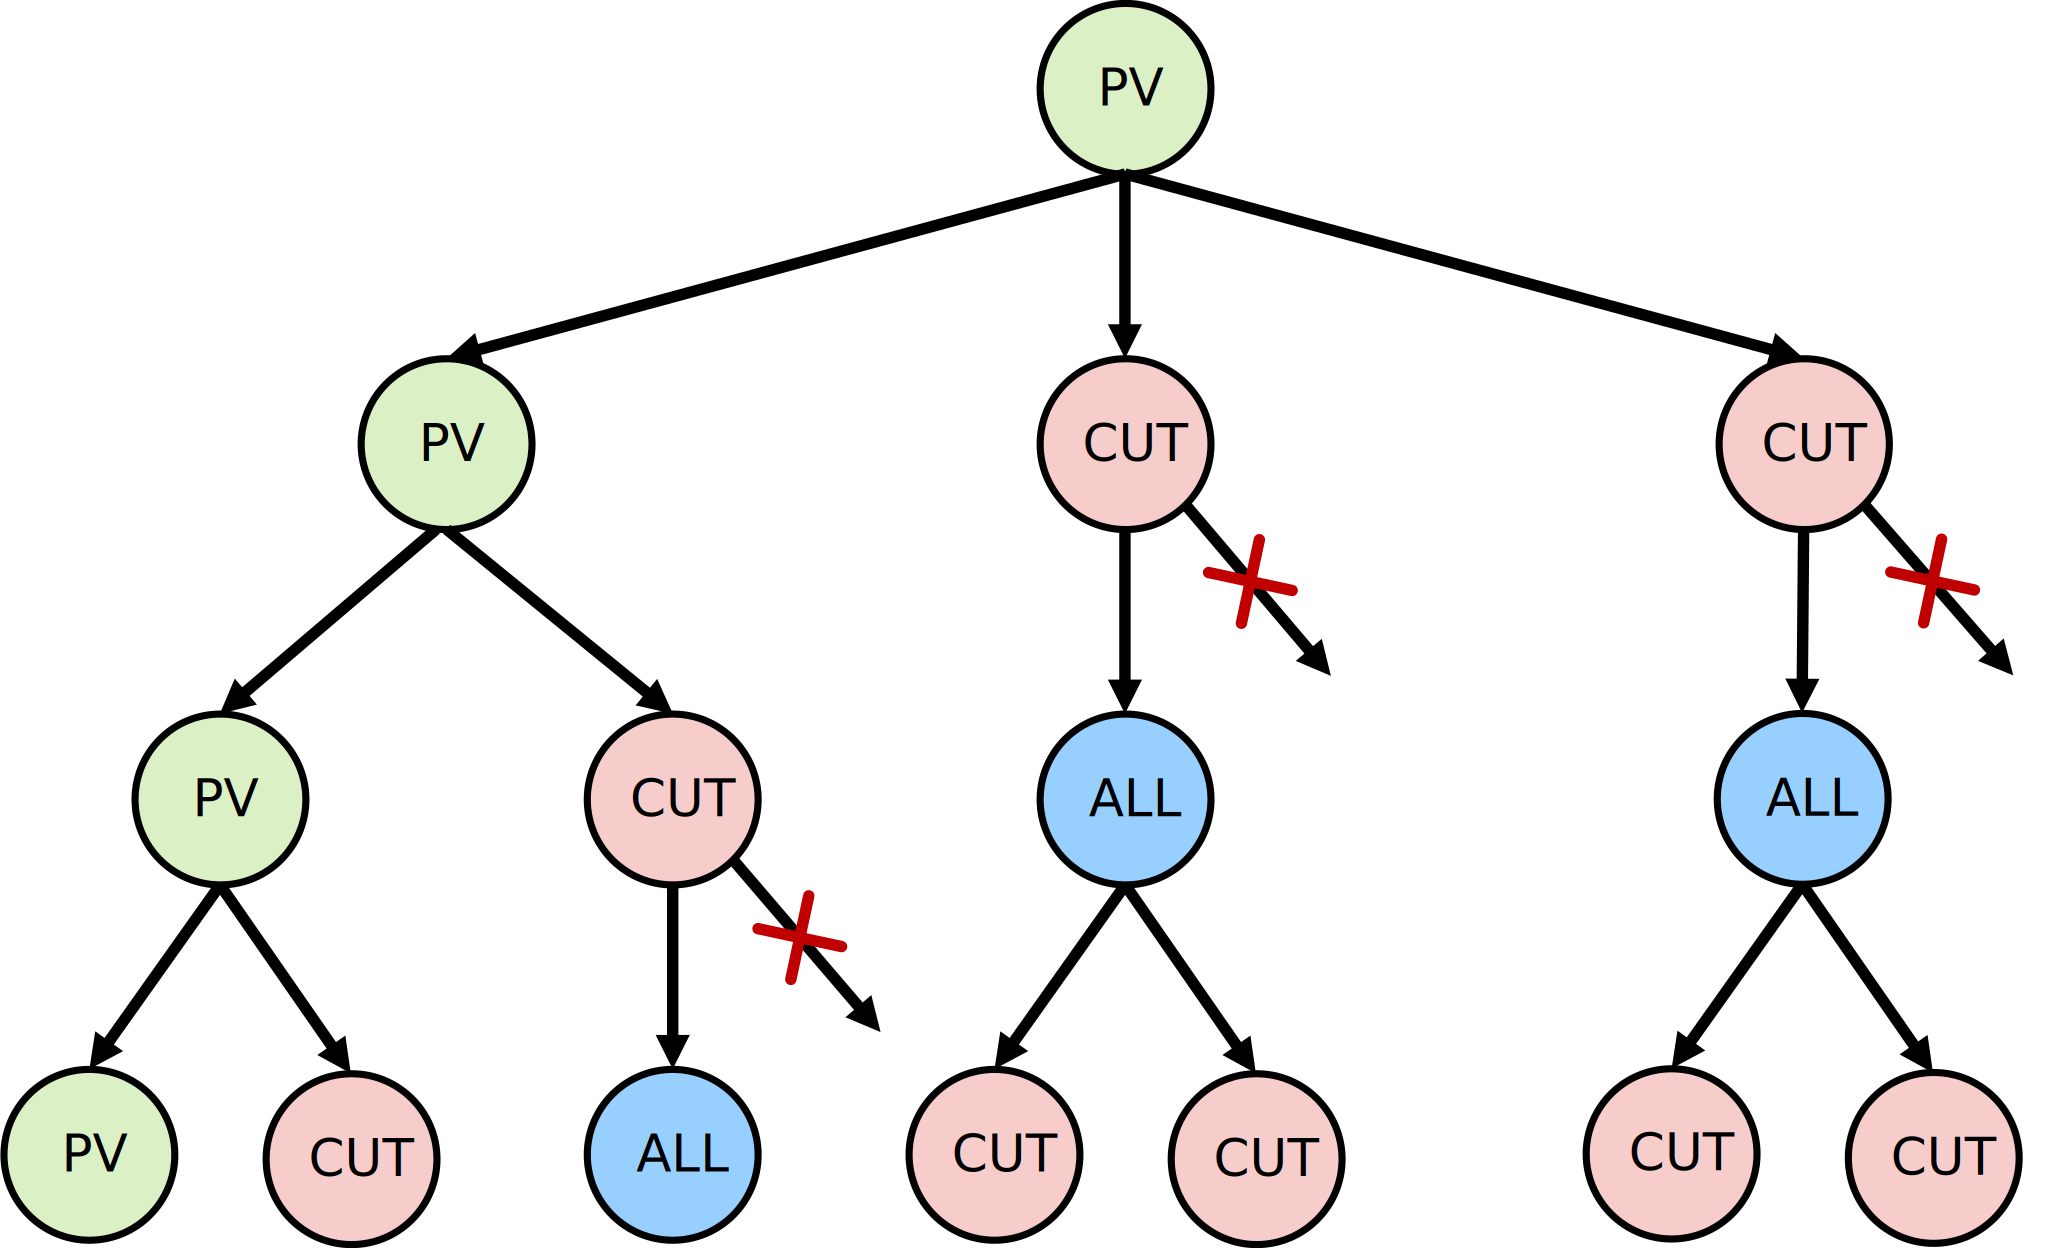
\includegraphics[width=0.695\textwidth]{res/pictures/minimal-search-tree.pdf}
    \caption{Minimaler Suchbaum bei der Alpha-Beta Suche}
    \label{fig:minimal-search-tree}
\end{figure}

\vspace*{-5cm}

\pagebreak

\begin{itemize}
    \item \labeltext{\emph{\acs{PV}-Knoten}}{text:pv-node} oder \emph{Typ-1-Knoten}: Die \ac{PV} ist eine Sequenz an Aktionen, bei denen beide Spieler immer die für sich beste Aktion wählen. Es handelt es also um den \enquote{perfekten} Spielverlauf, bei dem kein Pruning stattfinden kann. \cite[S. 316f.]{2005.EnhancedForwardPruning}
    \item \vspace*{-0.125cm} \labeltext{\emph{Cut-Knoten}}{text:cut-node} oder \emph{Typ-2-Knoten}: Sind Knoten, bei denen ein $\beta$-Cutoff stattgefunden hat, \dash es gab eine Suche mit den Grenzen $\left[\alpha, \beta\right]$ und der Wert war $\ge \beta$. Somit wurde in diesem Teilbaum für einen Spieler eine Aktion gefunden, die zu gut war, sodass der andere Spieler vorher eine andere Aktion auswählen wird, damit das Spiel überhaupt nicht in den Zustand dieses Knotens kommen kann. \cite[S. 324]{1975.AlphaBeta}
    \item \vspace*{-0.125cm} \labeltext{\emph{All-Knoten}}{text:all-node} oder \emph{Typ-3-Knoten}: Während der Suche aller Kinderknoten wurde kein Spielzustand gefunden, der besser als ein anderer Spielzustand, welchen der aktuelle Spieler durch das Ausführen einer anderen Aktion in einem anderem Teil des Suchbaums erreichen konnte. Bei einer Suche mit Grenzen $\left[\alpha, \beta\right]$ war die Evaluation aller Kinderknoten also $\le \alpha$. \cite[S. 446]{1985.ParallelAlphaBeta}
\end{itemize}

\vspace*{-0.13cm}

Mithilfe dieser Knotentypen lässt sich der minimale für Alpha-Beta-Pruning benötigte Suchbaum aufstellen \cite[S. 8]{1991.SingleAgentGameTreeSearch}. Dieser ist in Abbildung \ref{fig:minimal-search-tree} visualisiert. Da Alpha-Beta als Tiefensuche agiert, werden immer zuerst alle \hyperref[text:pv-node]{\acs{PV} Aktionen / Knoten} durchsucht. Jeder \hyperref[text:pv-node]{\emph{\acs{PV}-Knoten}} hat dabei immer genau einen weiteren \hyperref[text:pv-node]{\emph{\acs{PV}-Knoten}} sowie mehrere \hyperref[text:cut-node]{\emph{Cut-Knoten}} als Kinder. Die \hyperref[text:cut-node]{\emph{Cut-Knoten}} erzeugen dabei einen Teilbaum, bei dem sich immer wieder \hyperref[text:cut-node]{\emph{Cut-Knoten}} und \hyperref[text:all-node]{\emph{All-Knoten}} abwechseln. Bei \hyperref[text:cut-node]{\emph{Cut-Knoten}} muss immer nur das erste Kind durchsucht werden, während bei allen anderen Kinderknoten ein $\beta$-Cutoff stattfinden kann. Bei \hyperref[text:all-node]{\emph{All-Knoten}} müssen immer alle Kinderknoten durchsucht werden.

\acl{PVS} setzt an dieser Stelle an, indem versucht wird den minimalen Suchbaum auch während der Suche zu erhalten. Dazu wird die Alpha-Beta-Suche mit einer iterativen Tiefensuche kombiniert, \dash zuerst wird der gesamte Suchbaum mit Tiefe 1 durchsucht, dann mit Tiefe 2 und so weiter. Dieser Vorgang wiederholt sich, bis die Suchzeit vorbei ist. In jeder Iteration, wird dabei in jeder Ebene die beste gefundene Aktion, die \acl{PV}, gespeichert. In der nächsten Iteration wird dann davon ausgegangen, dass es sich bei der \acl{PV} der vorherigen Suche auch weiterhin um die \acl{PV} handelt, auch wenn nun eine Ebene tiefer gesucht wird. Sollte dies der Fall sein, können sehr große Teilbereiche des Baums schnell geprunt werden. Die iterative \ac{PVS} Tiefensuche ist dabei durch die größere Anzahl an geprunten Knoten im Regelfall schneller als die Alpha-Beta Suche mit einer festen Tiefe \cite[S. 13]{2017.Minimax}.

\begingroup

\setlength{\textfloatsep}{0pt}
\setlength{\intextsep}{0pt}

\refstepcounter{lstlisting}
\addcontentsline{lol}{lstlisting}{\protect\numberline{\thelstlisting}Pseudocode vom Principal-Variation-Search Algorithmus}

\begin{algorithm}[!ht]
    \caption{Pseudocode vom Principal-Variation-Search Algorithmus}
    \label{algo:principal-varation-search}
    \begin{algorithmic}[1]
        \Function{pvs}{$game$,\, $\alpha$,\, $\beta$,\, $depth$}
        \If{$depth == 0$ oder $game$ ist Terminalzustand}
        \State \Return $color\ \cdot $ \Call{evaluation}{$game$} \Comment{$max$-Player $color = 1$, sonst $-1$}
        \EndIf
        \For{each valid $action$ of $game$}
        \State $game.$\Call{do\_action}{$action$}
        \If{$action$ ist erste Aktion} \Comment{$\acs{PV}$-Action}
        \State $value = -$\Call{pvs}{$game$,\, $-\beta$,\, $-\alpha$,\, $depth - 1$} \label{alg:pvs-line-8}
        \Else
        \State $value = -$\Call{pvs}{$game$,\, $-\alpha - 1$,\, $-\alpha$,\, $depth - 1$} \Comment{\small \acf{ZWS}} \label{alg:pvs-line-10}
        \If{$\alpha < value < \beta$}
        \State $value = -$\Call{pvs}{$game$,\, $-\beta$,\, $-\alpha$,\, $depth - 1$} \label{alg:pvs-line-12}
        \EndIf
        \EndIf
        \State $game.$\Call{undo\_action}{$action$}
        \If{$value \ge \beta$}
        \State \Return $\beta$ \Comment{$\beta$-Cutoff}
        \EndIf
        \State $\alpha = \max\left(\alpha, value\right)$ \label{alg:pvs-line-19}
        \EndFor
        \EndFunction
    \end{algorithmic}
\end{algorithm}

\endgroup

In Pseudocode \ref{algo:principal-varation-search} ist die \ac{PVS}-Suche abgebildet. Alle Aktionen werden bei jeden Methodenaufruf so angeordnet, dass die \acl{PV} der vorherigen Suche die erste Aktion ist. Da dort ein \hyperref[text:pv-node]{\emph{\acs{PV}-Knoten}} erwartet wird, findet eine Suche mit dem normalen $\alpha$-$\beta$-Fenster statt (\hyperref[alg:pvs-line-8]{Zeile 8}). In allen anderen Fällen soll so schnell wie möglich bewiesen werden, dass man sich nicht mehr in einem \hyperref[text:pv-node]{\emph{\acs{PV}-Knoten}} befindet. Dazu wird die untere Begrenzung des $\alpha$-$\beta$-Fensters auf die Evaluation gesetzt (\hyperref[alg:pvs-line-19]{Zeile 19}). Handelt es sich bei der ersten Aktion tatsächlich um die \acl{PV}, so müssten alle weiteren Aktionen schlechter sein und somit eine Evaluation $\le \alpha$ zurückgeben. Um dies so schnell wie möglich zu beweisen, wird eine \acf{ZWS}, eine Suche mit einem Fenster $\left[\alpha, \alpha + 1\right]$, ausgeführt (\hyperref[alg:pvs-line-10]{Zeile 10}) \cite[S. 317]{2005.EnhancedForwardPruning}. Dadurch, dass die obere Grenze mit $\alpha + 1$ so niedrig wie möglich ist, werden deutlich mehr $\beta$-Cutoffs produziert als mit dem normalen $\beta$ Parameter. Solange der tatsächliche Wert auch unterhalb von $\alpha$ liegt, stellt das kein Problem dar. Ist diese Annahme falsch, so muss die Suche mit dem normalen $\alpha$-$\beta$-Fenster erneut durchgeführt werden, um die tatsächliche Evaluation des Knotens zu erhalten (\hyperref[alg:pvs-line-12]{Zeile 12}) \cite{2002.PrincipalVariationSearch}. Ist die tatsächliche Evaluation besser als der derzeitige $\alpha$-Wert, so war auch die Annahme, dass die erste Aktion die \acl{PV} ist falsch und der Knoten wird als die neue \acl{PV} festgesetzt (\hyperref[alg:pvs-line-19]{Zeile 19}) \cite[S. 5]{1999.SolutionTreesGameTreeSearch}.

\vspace*{-5cm}

\pagebreak

Die gesamte Implementation des \ac{PVS}-Algorithmus zusammen mit allen nachfolgend vorgestellten Modifikationen ist in Anhang \ref{code:pvs-search} zu finden.

\subsection{Aktionen-Anordnung}

Die Effizient von Alpha-Beta-Pruning also auch dem \ac{PVS}-Spieler hängt in großen Teilen davon ab, ab wie vielen durchsuchten Aktionen ein $\beta$-Cutoff erzielt werden kann \cite{2003.AlphaBetaSearch}. Je schneller dies passiert, desto weniger Baumknoten müssen durchsucht werden, womit die Engine die gewonnene Zeit für eine tiefergehende Suche verwenden kann. Deshalb sollten die Aktionen in einer möglichst vorteilhaften Reihenfolge durchsucht werden. Bei \ac{PVS} wird dadurch, dass die vorherige \ac{PV} Aktion an erster Stelle steht, schon eine möglichst gute Reihenfolge sichergestellt. Jedoch sind nicht in allen Knoten solche vorherigen \ac{PV} Aktionen vorhanden, beispielsweise wenn eine neue Tiefe durchsucht wird. Aus diesem Grund ist es sinnvoll alle Aktionen basierend auf einer Heuristik in eine Durchsuchungsreihenfolge anzuordnen.

Dabei wird bewusst von einer Aktionen-Anordnung und nicht von einer Aktionen-Sortierung gesprochen. Während man jeder Aktion basierend auf der Heuristik einen Wert zuweisen und danach die gesamte Liste sortieren könnte, ist dies ineffizient. Bei einem $\beta$-Cutoff, welcher meistens bereits bei der ersten Aktion passiert, wird nur eine teilsortierte Liste an Aktionen benötigt. \cite{2022.MoveOrdering}

\refstepcounter{lstlisting}
\addcontentsline{lol}{lstlisting}{\protect\numberline{\thelstlisting}Pseudocode: Aspiration Windows}

\begin{algorithm}[!ht]
    \caption{Pseudocode: Aktionen-Anordnung}
    \label{algo:action-ordering}
    \begin{algorithmic}[1]
        \Function{score\_actions}{$game$,\, $actions$,\, $pv\_action$}
        \For{each valid $action$ of $actions$}
        \State $action.score \gets $ \Call{score\_single\_action}{$game$,\, $action$,\, $pv\_action$}
        \EndFor
        \EndFunction
        \Function{pick\_action}{$actions$,\, $start\_index$}
        \LineComment Einzelne Iteration von Selectionsort
        \For{each $i \coloneq start\_index + 1$ bis $len\left(actions\right)$}
        \If{$actions\left[i\right].score > actions\left[start\_index\right].score$}
        \State swap $actions\left[start\_index\right]$ und $actions\left[i\right]$
        \EndIf
        \State \Return $actions\left[start\_index\right]$
        \EndFor
        \EndFunction
    \end{algorithmic}
\end{algorithm}

Aus diesem Grund besteht die in Pseudocode \ref{algo:action-ordering} dargestellte Aktionen-Anordnung aus zwei Schritten. Vor dem eigentlichen \ac{PVS}-Algorithmus wird jeder Aktion mit \code{score\_actions} ein durch die Heuristik vergebener Wert zugewiesen. Während jeder \ac{PVS} Iteration wird dann mit \code{pick\_action} eine Iteration des Selektionsort Algorithmus ausgeführt, um die nächste Aktion zu erhalten. Obwohl die Zeitkomplexität von Selektionsort $\mathcal{O}\left(n^2\right)$ ist, wird der Sortieralgorithmus für eine Teilsortierung aufgrund der einfachen Implementierung bevorzugt.

Für die Aktionen-Anordnung stellt sich nun die Frage wie genau die Heuristik aussieht. In Schach werden hierfür beispielsweise Aktionen, bei denen eine andere Schachfigur geschlagen wird nach dem \ac{MVV-LVA} Prinzip angeordnet \cite[S. 72]{2002.FPGAMoveGenerator}. In Patchwork gibt es keine Aktionen, die den Spielzustand eindeutig verbessern, wie das Schlagen von Spielfiguren. Eine vollständige Analyse der entstehenden Ablagepläne wäre zu zeitaufwendig. Um dennoch keine zufällige Aktionsanordnung zu erhalten, werden die in »\nameref{section:auswertung-empirischer-daten}« Aufgenommenen empirischen Spieldaten verwendet.
\begin{equation}
    \label{eqn:action-value}
    \frac{|wins|}{|games|} + \varepsilon \cdot \sqrt[3]{\frac{\sum score}{|games|}}
\end{equation}

Jeder Aktion wird dazu eine Liste an Endergebnissen zugeordnet, welche entstanden sind, nachdem die Aktion innerhalb eines Spiels verwendet wurde. Mithilfe dieser Endergebnisse wird für jede Aktion mittels des Terms \ref{eqn:action-value} ein \enquote{Wert} zugeordnet. Der Term berechnet dabei die Winrate des Spielers zusammen mit einem kleinen Anteil aus der Kubikwurzel des tatsächlichen Endergebniswerts. Ziel ist durch die große Anzahl an empirischen Spielen eine Approximation des tatsächlichen Wertes einer \enquote{Aktion} zu erhalten. Da in den empirischen Daten nicht alle Aktionen verwendet wurden, werden in den Daten nicht vorkommende Flickenlegeaktionen durch die Werte aus der umliegenden Nachbarschaft interpoliert. Weiterhin sind die Werte dabei noch in Opening- und Endgame-Tabellen aufgeteilt. Ist eine Aktion in den empirischen Daten vor 50\% der Gesamtanzahl der \hyperref[text:ply]{\emph{Plys}} des Spiels ausgeführt worden, so wird der Wert mit in die Berechnung der Opening-Tabelle aufgenommen, andernfalls für die Endgame-Tabelle verwendet. Zuletzt wurden alle Werte mittels einer Min-Max-Normalisierung auf den Wertebereich $\left[-1, 1\right]$ skaliert. Für die tatsächliche Aktionen-Anordnung wird dann der Wert der Aktion zwischen Opening- und Endgame-Tabelle mittels der Position des Spielers auf dem Zeitplan linear interpoliert.

Um die Effektivität dieser Aktion-Wert-Tabellen zu überprüfen, sind die Werte der Flickenplatzierenaktionen als Heatmap auf dem Ablageplan aufgetragen. So sind in Abbildung \ref{fig:action-ordering-patch-17} und \ref{fig:action-ordering-patch-21} die Heatmaps der Flicken 17 und 21 zu sehen. Für die Erstellung wurde dabei für jedes Feld auf dem Ablageplan geschaut, welche Aktionen dieses Feld belegen, deren Werte aussummiert und anschließend durch die Anzahl geteilt. In den Grafiken ist links ist die Heatmap der Opening-Werte und rechts die der Endgame-Werte abgebildet.

\vspace*{-0.77cm}

\begin{figure}[!ht]
    \centering
    \begin{minipage}{.11\textwidth}
        \centering
        \includegraphics[width=\linewidth]{res/pictures/assets/17-front.png}
    \end{minipage}
    \begin{minipage}{.78\textwidth}
        \centering
        \includegraphics[width=\linewidth]{res/pictures/plots/17-action-ordering.pdf}
    \end{minipage}
    \begin{minipage}{.11\textwidth}
        \hfill
    \end{minipage}
    \vspace*{-0.32cm}
    \captionof{figure}{Heatmap des Flicken 17}
    \label{fig:action-ordering-patch-17}
\end{figure}

\vspace*{-0.36cm}

\begin{figure}[!ht]
    \centering
    \begin{minipage}{.11\textwidth}
        \centering
        \includegraphics[width=0.667\linewidth]{res/pictures/assets/21-front.png}
    \end{minipage}
    \begin{minipage}{.78\textwidth}
        \centering
        \includegraphics[width=\linewidth]{res/pictures/plots/21-action-ordering.pdf}
    \end{minipage}
    \begin{minipage}{.11\textwidth}
        \hfill
    \end{minipage}
    \vspace*{-0.32cm}
    \captionof{figure}{Heatmap des Flicken 21}
    \label{fig:action-ordering-patch-21}
\end{figure}

\vspace*{-0.14cm}

Der Flicken 17 wird im perfekten Patchwork Spiel zu Beginn des Spiels verwendet, da er sehr viel Knopfeinkommen für einen relativ geringen Preis liefert (siehe \ref{section-loesung-des-optimierungsproblems}). Auch in der Heatmap ist der Flicken deshalb in der Opening-Tabelle mit sehr positiven Werten vertreten, während der Flicken im Endgame durch die hohen Kosten als negativ angesehen wird. Auch die positionen Auf dem Ablageplan stimmen mit der menschlichen Position überein. Flicken 17 ist durch seine kantige Form besser in der Mitte unterzubringen als am Rand des Ablageplans.

Den Erwartungen nach sollte Flicken 21 durch das nicht vorhandene Knopfeinkommen generell weniger wert sein als Flicken 17. Diese Annahme wird auch durch die Heatmap widergespiegelt. Auch, dass die Positionen an den Rändern erwartungsgemäß bei Flicken 21 besser bewertet werden, wird in der Heatmap deutlich. Vor allem verbessert sich die Bewertung von Flicken 21 im späterem Spiel, da dort das Füllen des Ablageplans deutlich relevanter ist als ein nicht existierendes Knopfeinkommen.

Generell sie die Werte der Aktionen nicht perfekt. So müssten die Werte symmetrisch über den Ablageplan verteilt sein, da jeder Spielverlauf auch einfach in einer gedrehten/gespiegelten Form existiert. Dies ist jedoch wie zu erkennen nicht der Fall. Weiterhin sind die in Heatmap \ref{fig:action-ordering-special-patch} dargestellten Werte der Spezialflicken zwar wie zu erwarten generell positiv, wirken aber noch sehr zufällig verteilt.

\begin{figure}[!ht]
    \centering
    \begin{minipage}{.78\textwidth}
        \centering
        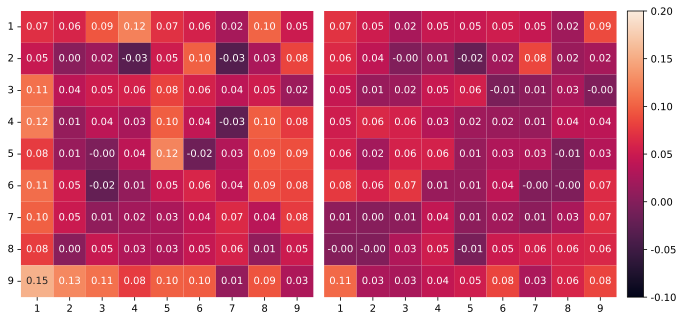
\includegraphics[width=\linewidth]{res/pictures/plots/special-action-ordering.pdf}
    \end{minipage}
    \captionof{figure}{Heatmap des Spezialflicken}
    \label{fig:action-ordering-special-patch}
\end{figure}

\subsection{Transposition Table und Zobrist Hashing}

Für die \ac{PVS} Suche müssen die \ac{PV} Aktionen für jeden Spielzustand gespeichert werden. Nur so kann in der nächsten Iteration diese wieder als erstes durchsucht werden. Weiterhin ist es sinnvoll alle bereits evaluierten Zustände während der Suche zwischenzuspeichern, sodass falls dieser Zustand in einem anderem Teilbaum erneut auftritt, einfach der Wert zurückgegeben werden kann, anstatt erneut den gesamten Teilbaum zu evaluieren. Die Transposition Table dient als Lösung für beide diese Anwendungsfälle.

Die in Patchwork verwendete Transposition Table besteht aus 2 Feldern. Zuerst wird das Alter der Transposition Table gespeichert. Dieses wird im jedem \hyperref[text:ply]{\emph{Ply}} inkrementiert, sodass alte Einträge der Tabelle erkannt und ignoriert werden können. Weiterhin gibt es eine $250\acsp{MiB}$ große Liste an Tabelleneinträgen. Um jeden Spielzustand einen Eintrag innerhalb der Liste zuzuordnen, muss eine Hashfunktion verwendet. Hierzu wird typischerweise ein \labeltext{\emph{Zobrist Hash}}{text:zobrist-hash} verwendet. Existiert eine Reihe an Elementen, wobei jedes Element nur endliche Menge an Zuständen annehmen kann, so kann jedem Element eine gleichverteilte Zufallszahl zugeordnet werden. Ein \hyperref[text:zobrist-hash]{\emph{Zobrist Hash}} dieser Elemente wird gebildet, indem alle Elemente mittels \ac{XOR} kombiniert werden. \cite[S. 3]{1990.ZobristHash}. Der Vorteil bei der Verwendung von \hyperref[text:zobrist-hash]{\emph{Zobrist Hashen}}  liegt in der schnellen Laufzeitperformance, da nur Indexzugriffe und \ac{XOR}-Bitoperationen verwendet werden.

\vspace*{-0.09cm}

\begin{figure}[!ht]
    \centering
    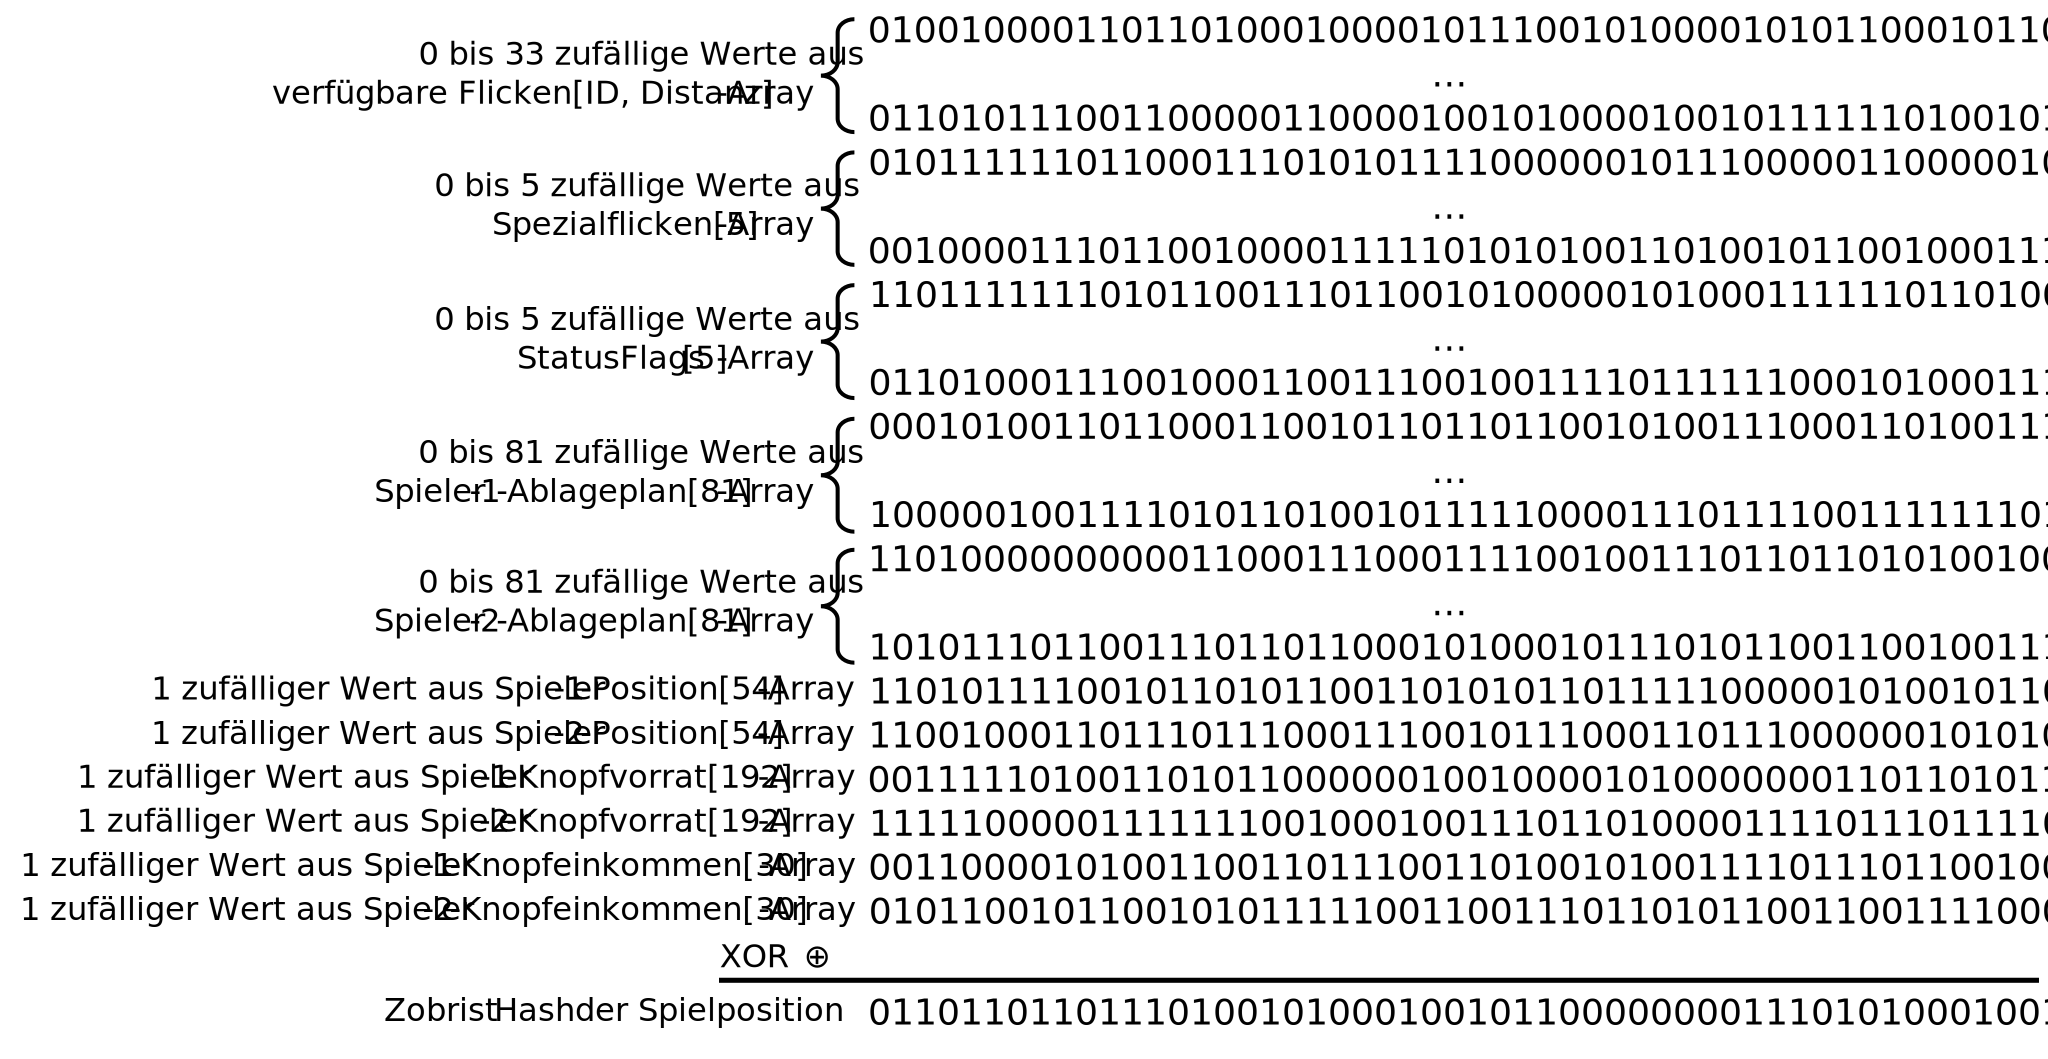
\includegraphics[width=\textwidth]{res/pictures/zobrist-hash.pdf}
    \vspace*{-0.35cm}
    \caption{Zobrist Hash}
    \label{fig:zobrist-hash}
\end{figure}

\vspace*{-0.2cm}

Der \hyperref[text:zobrist-hash]{\emph{Zobrist Hash}} in Patchwork setzt sich dabei aus den in Abbildung \ref{fig:zobrist-hash} gezeigten Bestandteilen zusammen. Da für alle diese Bestandteile aus dem \nameref{section:spieltheoretische-analyse} Kapitel Ober- und Untergrenzen bekannt sind, kann einfach im Voraus ein Array der benötigten Länge mit zufälligen Zahlen erstellt werden. Für den \hyperref[text:zobrist-hash]{\emph{Zobrist Hash}} wird dann einfach mit den Wert aus dem Spielzustand, \zB das aktuelle Knopfeinkommen, dieses Array indexiert. Gleichermaßen werden alle auf dem Ablageplan gefüllten Felder, die verfügbaren Flicken indexiert bei \ac{ID} und Distanz zur Spielfigur sowie alle anderen Bestandteile mit in den Zobrist-Hash aufgenommen.

\begin{table}[H]
    \centering
    \begin{tabular}{|c|l|}
        \hline
        Eintrag & Erläuterung                                                                                                      \\ \hline
        Key     & \ac{u64} mit \hyperref[text:zobrist-hash]{\emph{Zobrist Hash}} des Spielzustandes \emph{\acs{XOR}} das Data Feld \\ \hline
        Data    & Die Daten des Eintrags, codiert als ein \ac{u64} von \acs{MSB} nach \ac{LSB} mit:                                \\
                & \tabitem Evaluation (37 Bits): Die Evaluation des Spielzustandes                                                 \\
                & \tabitem Beste Aktion (17 Bits): Die beste Aktion ausgehend vom Spielzustand                                     \\
                & \tabitem Suchtiefe (8 Bits): Die Suchtiefe, bei der der Eintrag eingefügt wurde                                  \\
                & \tabitem Typ der Evaluation (2 Bits): untere Grenze, obere Grenze oder exakt                                     \\ \hline
        Age     & Das Alter des Eintrags.                                                                                          \\ \hline
    \end{tabular}
    \vspace{3pt}
    \caption{Transposition Table Eintrag}
    \label{tabelle:transposition-table-entry}
\end{table}

\vspace*{-0.2cm}

Ein Eintrag der Transposition Table ist in Tabelle \ref{tabelle:transposition-table-entry} darstellt. Zuerst wird der Schlüssel (Key) des Spielzustandes gespeichert, um mögliche Hashkollisionen zu erkennen, dann folgen alle relevanten Daten und zuletzt noch das Alter der Transposition Table zum Zeitpunkt des Einfügens, um alte Einträge zu erkennen und zu ignorieren. Die Daten sind dabei in einem besonderen Format gespeichert. Zuerst wird nicht der tatsächliche \hyperref[text:zobrist-hash]{\emph{Zobrist Hash}} als Key, sondern eine \ac{XOR}-Kombination mit den Daten als Schlüssel gespeichert. Weiterhin sind alle Daten in einen \ac{u64} codiert, anstatt diese in einzelnen Feldern zu speichern. All diese Modifikationen dienen dazu, Lockless Hashing zu unterstützen. Die \ac{PVS} Suche soll auch parallel Ablaufen können. Dazu muss die Transposition Table über mehrere Threads geteilt werden. Die geteilte Transposition Table sollte dabei möglichst ohne Locks auskommen, da das häufige Sperren und Freigeben einzelner Einträge ein Performanceoverhead ist.

\begin{lstlisting}[
    label={code:lockless-hashing},
    caption={Einfügen und Lookup bei Lockless Hashing},
    captionpos=b,
    language=Rust,
    escapeinside={<*}{*>},
    numbers=none]
index = zobrist_hash % TABLE_SIZE;

// Einfügen
tt_table[index].<*key*>  = zobrist_hash ^ data;
tt_table[index].data = data;

// Lookup
if (tt_table[index].<*key*> ^ tt_table[index].data == zobrist_hash) {
   // Eintrag gefunden
}
\end{lstlisting}

Lockless Hashing umgeht das Problem von Synchronisation, indem ein Eintrag wie in Quellcode \ref{code:lockless-hashing} eingefügt wird. So kann bei der Lookup-Operation einfach der Key mit dem Data Feld durch ein \ac{XOR} zurück in den \hyperref[text:zobrist-hash]{\emph{Zobrist Hash}} umgewandelt werden. Dadurch, dass in der Lookup-Operation beide Felder verwendet werden, kann so sichergestellt werden, dass Key und Data auch tatsächlich übereinstimmen. Sollte ein anderer Thread gleichzeitig auch nur eines der Felder ändern, so würde die Überprüfung fehlschlagen. Aus diesem Grund können mehrere Threads gleichzeitig den Eintrag lesen und schreiben, ohne dass ein korrupter Zustand aus der Transposition Table ausgelesen werden kann. \cite{2002.LocklessTT}

Das Daten Feld beinhaltet die Evaluation des Spielzustandes, sodass diese in einem anderem Teilbaum wiederverwendet werden kann. Weiterhin wird die beste von diesem Zustand ausgehende Aktion, also die \ac{PV}-Aktion gespeichert. Falls diese nicht bekannt ist, werden die Bits der \emph{Null}-ActionId gespeichert. Die Suchtiefe ist wie das Alter eines Eintrags für Lookup und Ersetzung von Einträgen relevant. Weiterhin wird ein EvaluationTyp gespeichert, welcher einer von drei möglichen Zuständen annehmen kann:

\begin{itemize}
    \item Exakt: Der gespeicherte Spielzustand ist ein \hyperref[text:pv-node]{\acs{PV}-Knoten} und die Evaluation ist somit exakt.
    \item Untere Grenze / Fail-High: Der Knoten ist ein \hyperref[text:cut-node]{Cut-Knoten} und somit ist die gespeicherte Evaluation nur eine untere Grenze für den tatsächlichen Wert des Spielzustands.
    \item Obere Grenze / Fail-Low: Der Knoten ist ein \hyperref[text:all-node]{All-Knoten}. Die Evaluation ist somit nur eine untere Grenze und der tatsächliche Wert kann noch niedriger sein.
\end{itemize}

Für das Einfügen neuer Einträge in die Transposition Table müssen die in Pseudocode \ref{algo:transposition-table-overwrite} dargestellte Bedingungen erfüllt sein. So können leere Einträge oder Einträge aus einem vorherigen \hyperref[text:ply]{\emph{Ply}} immer überschrieben werden. Weiterhin werden alte Einträge überschrieben, falls der neu einzufügende Eintrag für die Evaluation tiefer gesucht hat als der alte Eintrag. Falls also ein bestehender Eintrag existiert, welcher nach der Spielposition noch 3 weitere Ebenen für die Evaluation gesucht hat, wird dieser durch einen neuen Eintrag mit Suchtiefe 4 oder mehr überschrieben. Weiterhin werden Einträge, die nur eine obere oder untere Grenze besitzen durch exakte Evaluationen ausgetauscht.

\pagebreak

\refstepcounter{lstlisting}
\addcontentsline{lol}{lstlisting}{\protect\numberline{\thelstlisting}Pseudocode: Aspiration Windows}

\begin{algorithm}[!ht]
    \caption[Pseudocode: Transposition Table Überschreiben]{Pseudocode: Logik zum Überschreiben von Transposition Table Einträgen}
    \label{algo:transposition-table-overwrite}

    \begin{algorithmic}[1]
        \State \textbf{if} entry.key == 0 \textbf{then}
        \State \hspace*{\algorithmicindent} \Return \emph{Überschreiben} \Comment{Eintrag ist leer}
        \State \textbf{if} entry.age < current\_age \textbf{then}
        \State \hspace*{\algorithmicindent} \Return \emph{Überschreiben} \Comment{Alte Einträge überschreiben}
        \State \textbf{if} entry.data.depth <= new\_depth \textbf{then}
        \State \hspace*{\algorithmicindent} \Return \emph{Überschreiben} \Comment{Einträge mit geringerer Tiefe überschreiben}
        \State \textbf{if} entry.data.depth == new\_depth
        \State \hskip1em \textbf{and} entry.age == current\_age
        \State \hskip1em \textbf{and} entry.data.evaluation\_type != EvaluationType::Exact
        \State \hskip1em \textbf{and} new\_evaluation\_type == EvaluationTyp::Exact \textbf{then}
        \State \hspace*{\algorithmicindent} \Return \emph{Überschreiben} \Comment{Nicht \acs{PV} Einträge überschreiben}
        \State \Return \emph{Nicht Überschreiben}
    \end{algorithmic}
\end{algorithm}

Um den in Abschnitt \ref{subsection:zustandsraum-komplexitaet} aufgezeigten großen Zustandsraum wenigstens teilweise entgegenwirken, wird das Einfügen eines Eintrags noch erweitert. Wenn eine Spielposition erreichbar ist, so ist die gleiche Spielposition mit gedrehten und gespiegelten Ablageplänen beider Spieler ebenso erreichbar und besitzt die gleiche Evaluation. Aus diesem Grund werden all diese symmetrischen Spielpositionen gleichzeitig mit dem originalen Eintrag in die Transposition Table eingefügt.

Um einen Eintrag in der Transposition Table nachzuschauen (Quellcode \ref{code:probe-hash-entry}), muss einfach mit der zuvor vorgestellten Routine überprüft werden, ob der Transposition Table Eintrag mit dem Spielstand übereinstimmt. Ist dies der Fall, muss die Suchtiefe des Eintrags größer gleich der noch zu durchsuchenden Tiefe sein. Es macht beispielsweise keinen Sinn einen Transposition Eintrag zu verwenden, der nur noch eine ebene weitergesucht hat, wenn die eigene Suchfunktion noch mindestens 2 Ebenen tiefer suchen muss. Weiterhin muss beim Lookup auch der EvaluationTyp beachtet werden. Ist der EvaluationTyp ein exakter Wert, kann dieser eingeschränkt auf das $\alpha$-$\beta$-Fenster zurückgegeben werden. Ist nur eine obere Grenze für die Evaluation gespeichert, kann diese nur zurückgegeben werden, wenn sich diese obere Grenze auch unterhalb des $\alpha$-$\beta$-Fensters, also unterhalb von $\alpha$ befindet. Analog verhält es sich mit einer unteren Grenze. Soll nur die \ac{PV}-Aktion aus der Transposition Table ausgelesen werden, sind alle Nebenbedingungen egal. Jedoch kann es dabei vorkommen, dass auch die invalide \emph{Null}-Aktion zurückgegeben wird, da die beste Aktion nicht bekannt ist.

\pagebreak

\lstinputlisting[
    label={code:probe-hash-entry},
    caption={Lookup in der Transposition Table},
    captionpos=b,
    language=Rust,
    firstline=0,
]{res/code/probe-hash-entry.rs}

\pagebreak

\subsection{Aspiration Windows}

Eine mögliche Verbesserung der Iterativen Tiefensuche liegt in der Verwendung von Aspiration Windows. Bei der einfachen Implementierung der Tiefensuche ist der initiale Aufruf der \ac{PVS}-Suche immer mit $\alpha = -\infty$ und $\beta = \infty$. Bei Aspiration Windows wird diese Annahme insofern aufgelockert, indem davon ausgegangen wird, dass sich der Wert der nächsten Suchiteration nicht viel von dem Wert der vorherigen Suche unterscheidet. Deshalb wird statt dem gesamten Bereich nur ein Fenster (Aspiration Window) der Größe $\Delta$ um den vorherigen Suchwert erkundet. \cite{2003.AspirationWindows}

Da das initiale Fenster deutlich schmaler ist, können während der Suche im Normalfall mehr $\beta$-Cutoffs erreicht werden, was somit gleichzeitig einer kürzeren Suche entspricht. In den meisten Fällen gibt die Suche mit dem Aspriation Window auch wieder einen Wert innerhalb des Fensters von $\alpha$ und $\beta$ zurück. Ist dies nicht der Fall, muss die Suche zwingend erneut mit einem breiterem Aspiration Window wiederholt werden, was ein Nachteil bei der Verwendung ist.

\refstepcounter{lstlisting}
\addcontentsline{lol}{lstlisting}{\protect\numberline{\thelstlisting}Pseudocode: Aspiration Windows}

\begin{algorithm}[!ht]
    \caption{Pseudocode: Iterative Tiefensuche mit Aspiration Windows}
    \label{algo:aspiration-window}
    \begin{algorithmic}[1]
        \Function{search}{$game$}
        \State $\alpha \gets $ Starting-$\alpha$,\ \ $\beta \gets $ Starting-$\beta$,\ \ $\Delta \gets $ Starting-$\Delta$
        \For{$depth \coloneq 0$ bis Maximaltiefe}
        \State $value \gets \Call{principal\_variation\_search}{$\alpha$,\,$game$,\,$\beta$}$
        \If{Suchzeit vorbei}
        \State \textbf{break}
        \ElsIf{$value \le \alpha$} \Comment{Aspriation Window Fail-Low}
        \State $\alpha = value - \Delta$
        \State $\beta = (\alpha + \beta) / 2$ \Comment{$\beta$ in die Mitte des Fenster}
        \State $\Delta = \sfrac{4}{3}\cdot \Delta$
        \State \textbf{continue}
        \ElsIf{$value \ge \beta$} \Comment{Aspriation Window Fail-High}
        \State $\beta = value + \Delta$
        \State $\Delta = \sfrac{4}{3}\cdot \Delta$
        \State \textbf{continue}
        \EndIf
        \State $\Delta = $ \Call{new\_delta}{$value$,\, Starting-$\Delta$}
        \State $\alpha = value - \Delta$
        \State $\beta = value + \Delta$
        \EndFor
        \EndFunction
    \end{algorithmic}
\end{algorithm}

Wird ein Wert unterhalb von $\alpha$ zurückgegeben, handelt es sich um einen \emph{Fail-Low}, ist der Wert oberhalb von $\beta$, ist es ein \emph{Fail-High} Fall. Um im solch einen Failing-Fall möglichst effizient zu agieren, wird das Aspiration Window oftmals mit einem exponentiellen Backoff breiter gemacht, bis der Wert der Suche innerhalb des Fensters liegt. Die im Pseudocode \ref{algo:aspiration-window} verwendeten Werte für die Anpassung von $\alpha$, $\beta$ und $\Delta$ entsprechen dabei den Werten, welche in Stockfish verwendet werden, was eine der besten Schach-Computerspielengines ist \cite{2024.StockfishBackoff} \cite{2024.Stockfish}. Aus diesem Grund verwendet der \ac{PVS}-Spieler den gleichen exponentiellen Backoff. Bei einer einfachen Mimimax-Suche lässt sich in einem Fail-Fail die Fenstergrenze, welche nicht fehlgeschlagen ist, immer auf die andere Grenze setzten. Kommt es also zu einem Fail-High bei der Suche mit Aspiration Window $\left[\alpha, \beta\right]$, so könnte die nächste Suche mit $\left[\beta, \beta + \Delta\right]$ stattfinden. Bei der Suche des \ac{PVS}-Spielers ist dies aufgrund von Suchinstabilität nicht der Fall. Suchinstabilität heißt, dass eine wiederholte Suche eines Spielzustands nicht immer die gleiche Evaluation zurückgeben muss \cite{2003.SearchInstability}. Diese Suchinstabilität kann bereits durch die Verwendung der gespeicherten Evaluationen aus der Transposition Table entstehen \cite{2003.SearchInstability}. Im Falle der Aspiration Windows bedeutet dies, dass eine Suche, die vorher mit Fail-High abgebrochen wurde, in der darauffolgenden Suche einen Fail-Low erzeugen kann. Deshalb wird der Wert von $\beta$ im Pseudocode zum Beispiel nur in die Mitte des Fensters verschoben.

\subsection{Suchselektivität}

Shannon führt in seinem Wert \emph{\enquote{Programming a Computer for Playing Chess}} eine Klassifizierung der Suchmethoden in einem Spielbaum ein, die zwei Haupttypen umfasst: \textbf{Typ-A} ist eine vollständige Brute-Force-Suche durch den gesamten Baum bis zu einer gewissen Tiefe \cite[S. 8]{1950.ChessShannon}. Bei der \textbf{Typ-B} werden die Äste des Spielbaums so selektiv ausgewählt, dass interessante Teilbäume tiefer durchsucht werden und uninteressante Teilbäume nur reduziert oder gar nicht durchsucht werden.

Im Bereich der Sucherweiterungen werden in Schach normalerweise Aktionen wie das Schlagen von Schachfiguren oder Schachsetzten berücksichtigt \cite[S. 14]{1950.ChessShannon}\cite{2023.StockfishTerminology}\cite{2002.SearchExtensions}. Während solche Aktionen in Patchwork nicht existieren, gibt es zwei Ereignisse, die für einen Spieler besonders interessant sind: Das Erhalten des $7\times 7$ Sonderplättchens sowie das Legen eines Spezialflicken. Bei beiden Aktionen wird die Suche deshalb um eine Tiefenebene erhöht (Anhang \ref{code:pvs-search-extension}). Im Fall der Null-Fenster-Suche werden keine Sucherweiterungen angewendet.

\vspace*{-5cm}

\pagebreak

Für Patchwork sind Suchreduktionen im Bereich der Typ-B-Suche jedoch von größerer Bedeutung. Um bei Spielzuständen, die viele Aktionen erlauben und somit einen hohen Verzweigungsfaktor haben, den Suchaufwand möglichst minimal zu halten, sollte ein großer Teil der Aktionen nur reduziert durchsucht oder ganz weggelassen werden. Im \ac{PVS}-Spieler kommen hierzu zwei Konzepte zum Einsatz: \ac{LMR} und \ac{LMP}.

Bei einer Suche mit einigermaßen guter Zugreihenfolge tritt ein \hyperref[text:beta-cutoff]{\emph{Beta-Cutoff}} wenn überhaupt normalerweise am ersten \hyperref[text:pv-node]{\emph{\acs{PV}-Knoten}} auf \cite{2007.LMR}. Deswegen werden bei \ac{LMR} nur die ersten Aktionen mit der vollen Tiefe durchsucht und alle weiteren Aktionen werden insofern nichts interessantes passiert mit einer reduzierten Tiefe durchsucht. Als Nachteil muss aber bei einem zu guten Ergebnis über $\alpha$ der Teilbaum mit voller Tiefe erneut durchsucht werden \cite{2007.LMR}. Im \ac{PVS}-Spieler wird die Suche bei allen nicht \ac{PV}-Aktionen ab einer gewissen Tiefe auf ein Drittel der originalen Tiefe reduziert. Vorher wird die Suche immer um eine Ebene reduziert.

Bei \ac{LMP} wird ein noch drastischere Ansatz verfolgt, indem bestimmte Teilbäume gar nicht mehr anstatt nur reduziert durchsucht werden \cite{2023.StockfishTerminology}. Dabei handelt es sich um einen Tradeoff zwischen Suchgenauigkeit bzw. -stabilität und Zeit. Je mehr Aktionen \emph{geprunt}, also weggelassen werden, desto tiefer kommt die Suche. Gleichzeitig könnten aber so Teilbäume übersehen werden, welche einen besseren Spielverlauf beinhalten. Um die sehr große Anzahl an Aktionen, die bei einem Spielzustand auftreten können (1345) zu reduzieren, werden sehr viele Aktionen im \ac{PVS}-Spieler geprunt. Während in der ersten Ebene immer alle Aktionen betrachtet werden, wird in den späteren Tiefen immer nur sichergestellt, dass mindestens 3 Platzierungsmöglichkeiten für jeden Flicken überprüft werden. Die Auswahl dieser Aktionen basiert dabei auf der Bewertung der Aktionen-Anordnung. Die spezifischen Pruning-Werte wurden ermittelt, indem verschiedene Konfigurationen für die Starttiefe und die Anzahl an Platzierungsmöglichkeiten pro Flicken mit dem klassischen Alpha-Beta-Minimax-Algorithmus (wie in \ref{algo:minimax-alpha-beta}) gegeneinander spielten. Dabei wurden die besten Werte für den \ac{PVS}-Spieler übernommen.

\pagebreak

\subsection{Lazy-SMP}

Der bisher beschriebene \ac{PVS}-Spieler läuft Single-Threaded ab. Da heutige Computer mehrere Kerne besitzen, sollten diese aber auch verwendet werden. Für Mimimax sowie davon abgeleitete Algorithmen existiert dazu eine einfache aber gleichzeitig so effektive Parallelisierungsmöglichkeit, dass selbst die besten Schachengines diese verwenden \cite{2016.Stockfish7} \cite[S. ]{2016.ParallelChessEngine}.

Bei Lazy \ac{SMP}, werden $n$ parallele unabhängige Suchen gleichzeitig gestartet, welche sich nur die Transposition Table teilen. Dadurch, dass alle bereits durchsuchten Spielzustände in die Transposition Table eingefügt werden, wird sichergestellt, dass Spielzustände, welche zuvor von Threads erkundet wurden, nicht erneut durchsucht werden müssen. Dadurch, dass die Transposition Table bereits Lockless Hashing verwendet, können im Code einfach neue Threads gestartet werden, ohne dass weitere Synchronisationsmechanismen eingebaut werden müssen. Nachdem die Zeit abgelaufen ist, werden alle Threads gestoppt und die \ac{PV} Aktion aus der Transposition Table ausgelesen.

\section{Ansatz D: Monte Carlo Tree Search}
\label{section:erstellung-ansatz-c}

TODO:

\begin{itemize}
    \item Normaler MCTS
    \item UCT (Upper Confidence Bound for Trees)
    \item Parallel (Root und Leaf)
    \item Tree Reuse
    \item Evaluator (WinLoss, Score) -> In Eval genauer betrachten
\end{itemize}

\section{Ansatz E: AlphaZero}
\label{section:erstellung-ansatz-d}

TODO:

\begin{itemize}
    \item Änderungen Gegenüber MCTS / Generelle Funktionsweise
    \item Kodierung des Spielzustandes
    \item Netzwerk-Architektur
    \item Parallelization with Virtual Loss
    \item Training-Loop
\end{itemize}

\subsubsection*{Kodierung des Spielzustandes}

\begin{figure}[!ht]
    \centering
    \vspace*{-1.75cm}
    \includegraphics[width=\textwidth]{res/pictures/patch-zero-state.pdf}
    \caption{Zustandskodierung von PatchZero}
    \label{fig:patch-zero-state}
\end{figure}

TODO: LSTM Bild

\pagebreak

\subsubsection*{Netzwerk-Architektur}

\cite{2018.Lc0AlphaZero}
\cite{2019.SqueezeandExcitation}
\cite{2020.Lc0NetworkTopology}

\begin{figure}[!ht]
    \centering
    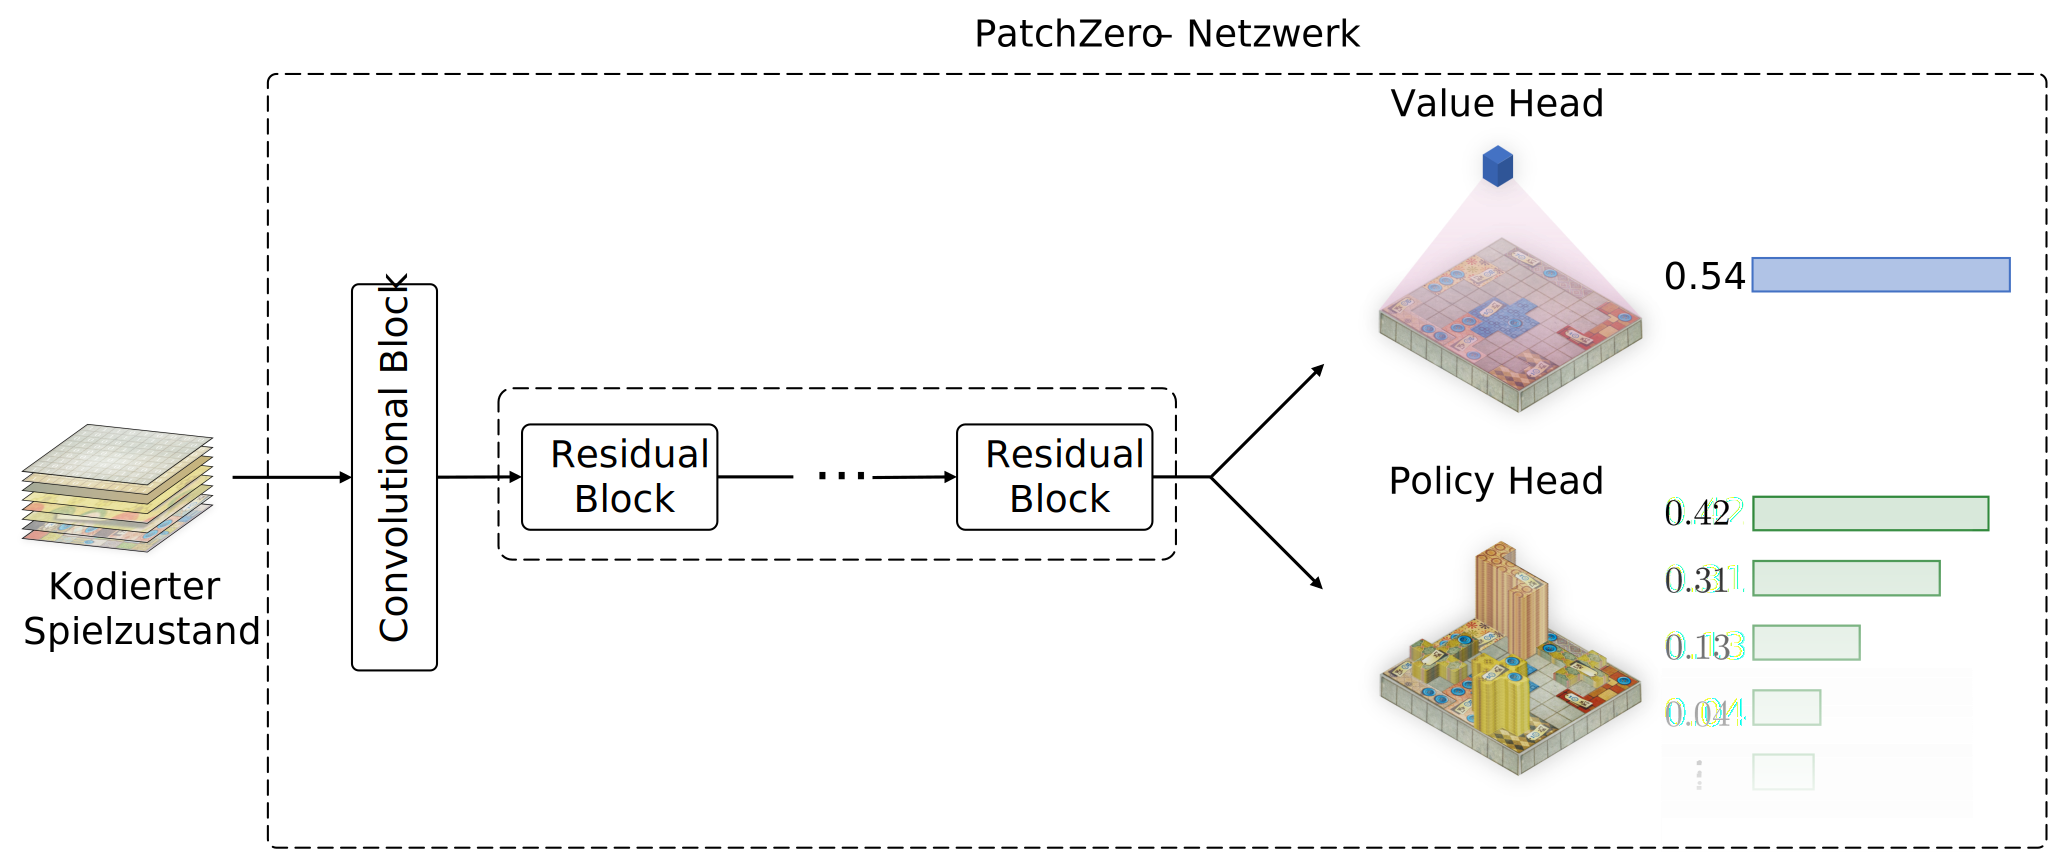
\includegraphics[width=\textwidth]{res/pictures/patch-zero-architecture.pdf}
    \caption{Architektur von PatchZero}
    \label{fig:patch-zero-architecture}
\end{figure}

TODO:

\begin{wrapfigure}{r}{0.25\textwidth}
    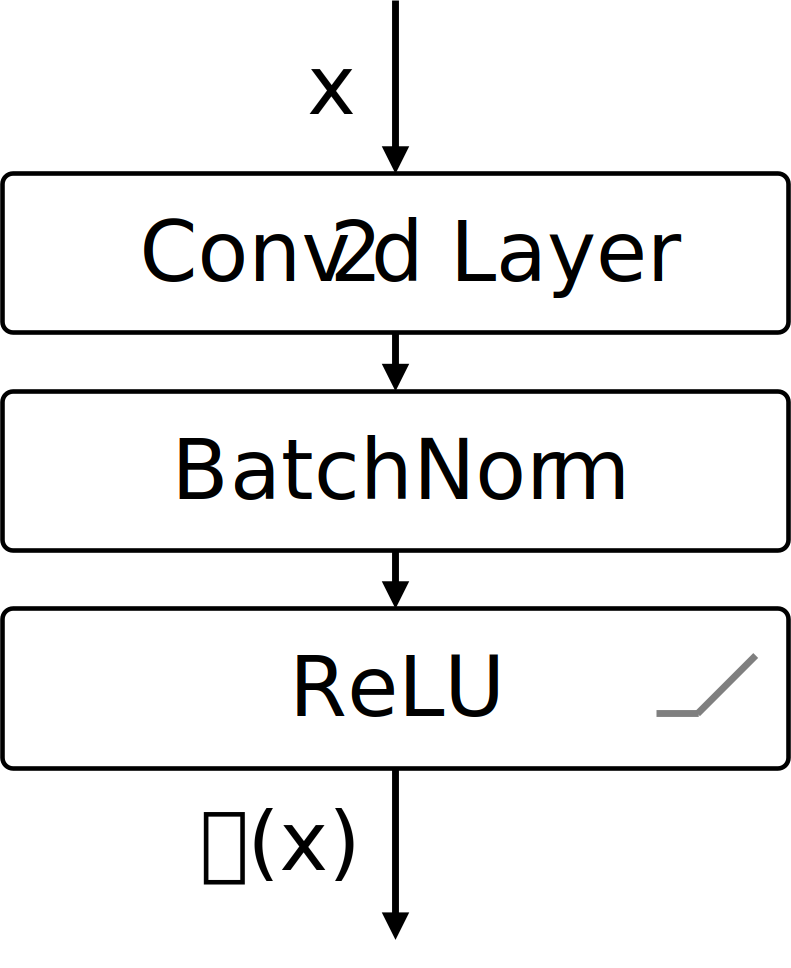
\includegraphics[width=0.2\textwidth]{res/pictures/conv-block.pdf}
    % \vspace{-10pt}
    % Das folgende ist ein Trick, um "Abbilgung x.y" in eine
    % eigene Zeile zu packen. Der Text zwischen [ und ] steht
    % im Abbildungsverzeichnis. Der Text darunter wird
    % tatsächlich angezeigt.
    \centering
    \caption[Convolutional Block]{\unskip}
    Convolutional Block
    \label{fig:conv-block}
\end{wrapfigure}

TODO:

\begin{wrapfigure}{l}{0.3\textwidth}
    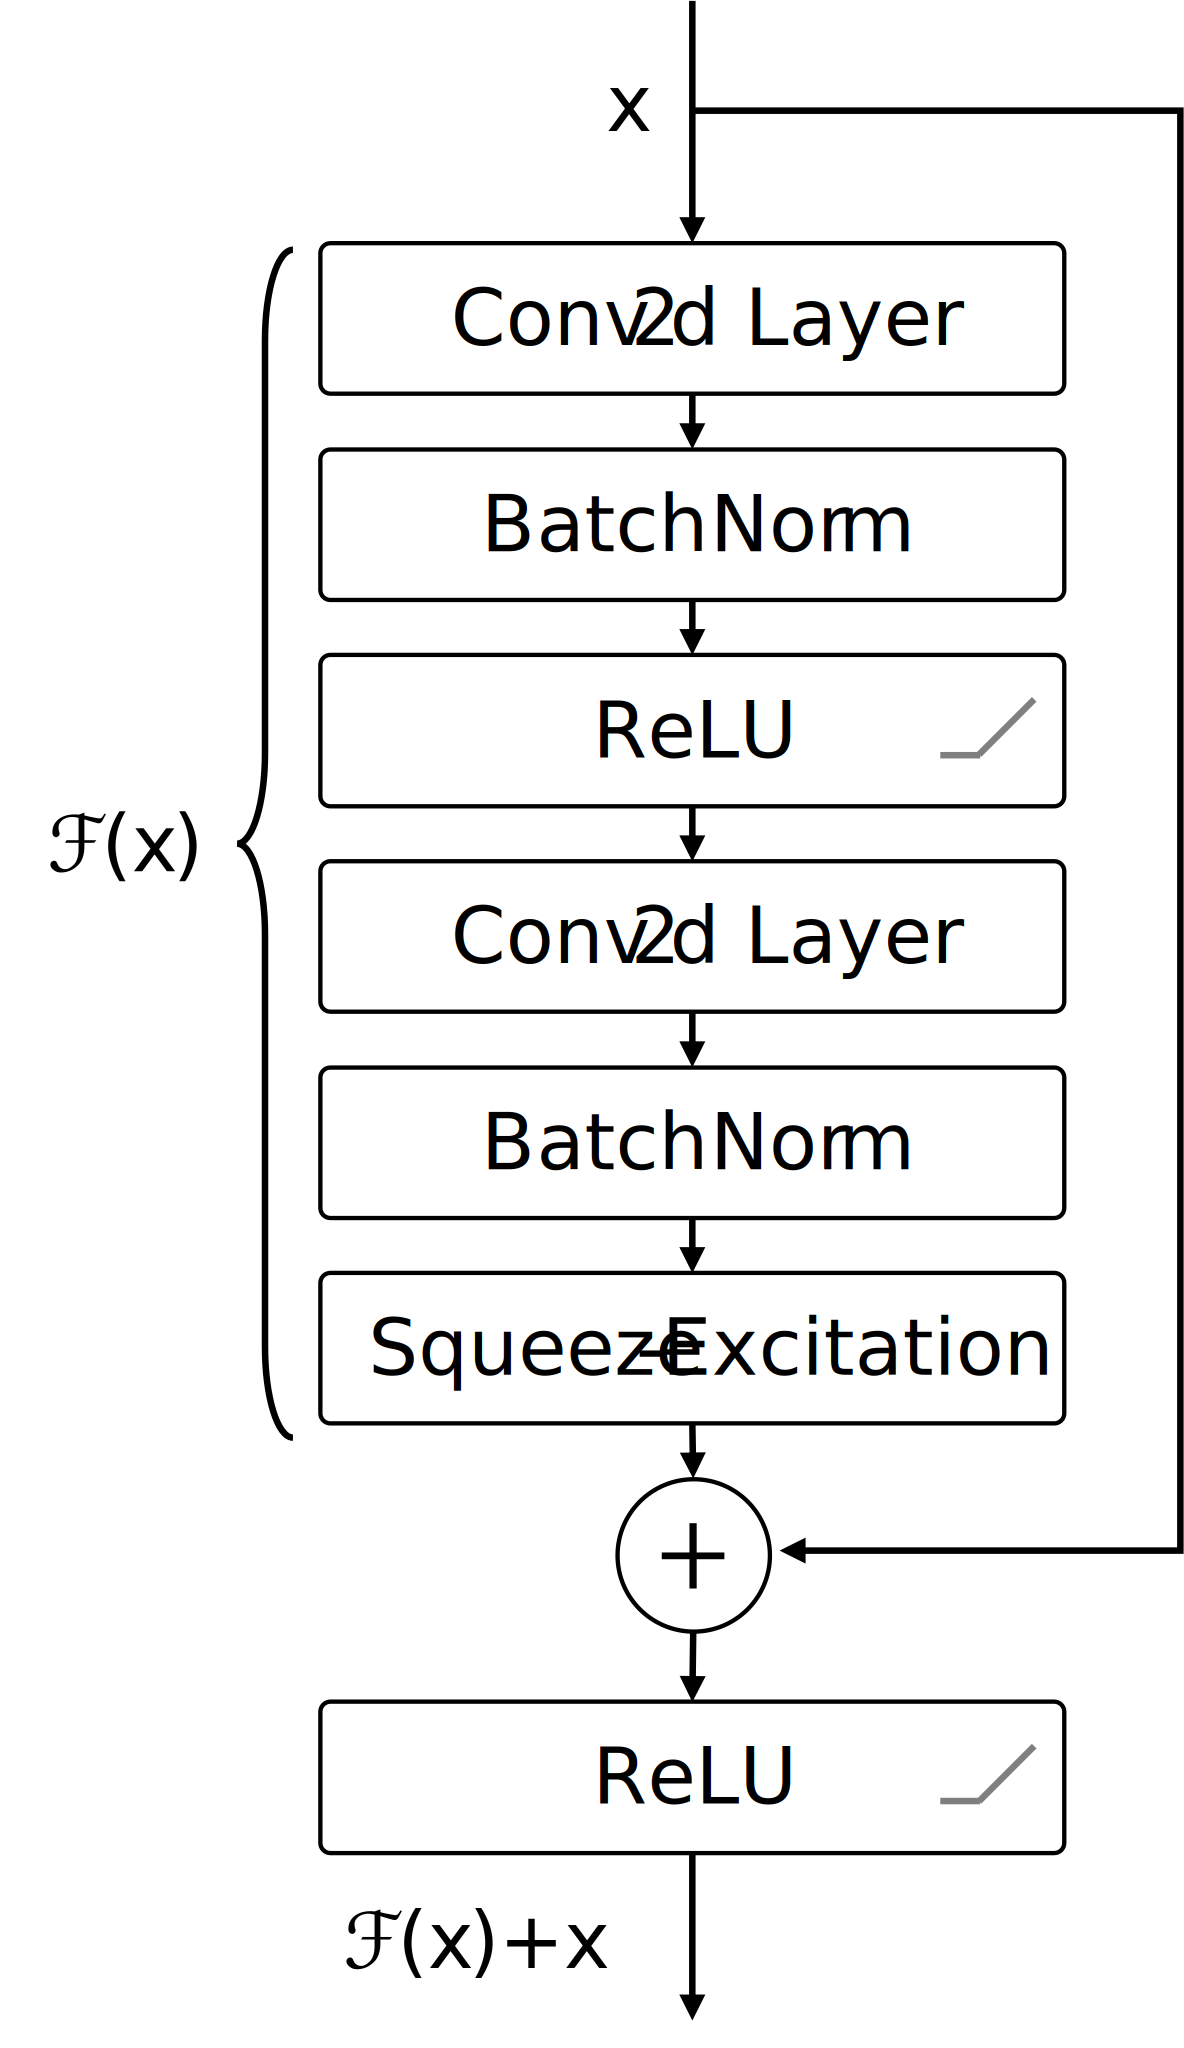
\includegraphics[width=0.25\textwidth]{res/pictures/res-block.pdf}
    % \vspace{-10pt}
    % Das folgende ist ein Trick, um "Abbilgung x.y" in eine
    % eigene Zeile zu packen. Der Text zwischen [ und ] steht
    % im Abbildungsverzeichnis. Der Text darunter wird
    % tatsächlich angezeigt.
    \centering
    \caption[Residual Block]{\unskip}
    Residual Block
    \label{fig:resblock}
\end{wrapfigure}

TODO:

\begin{wrapfigure}{r}{0.35\textwidth}
    \centering
    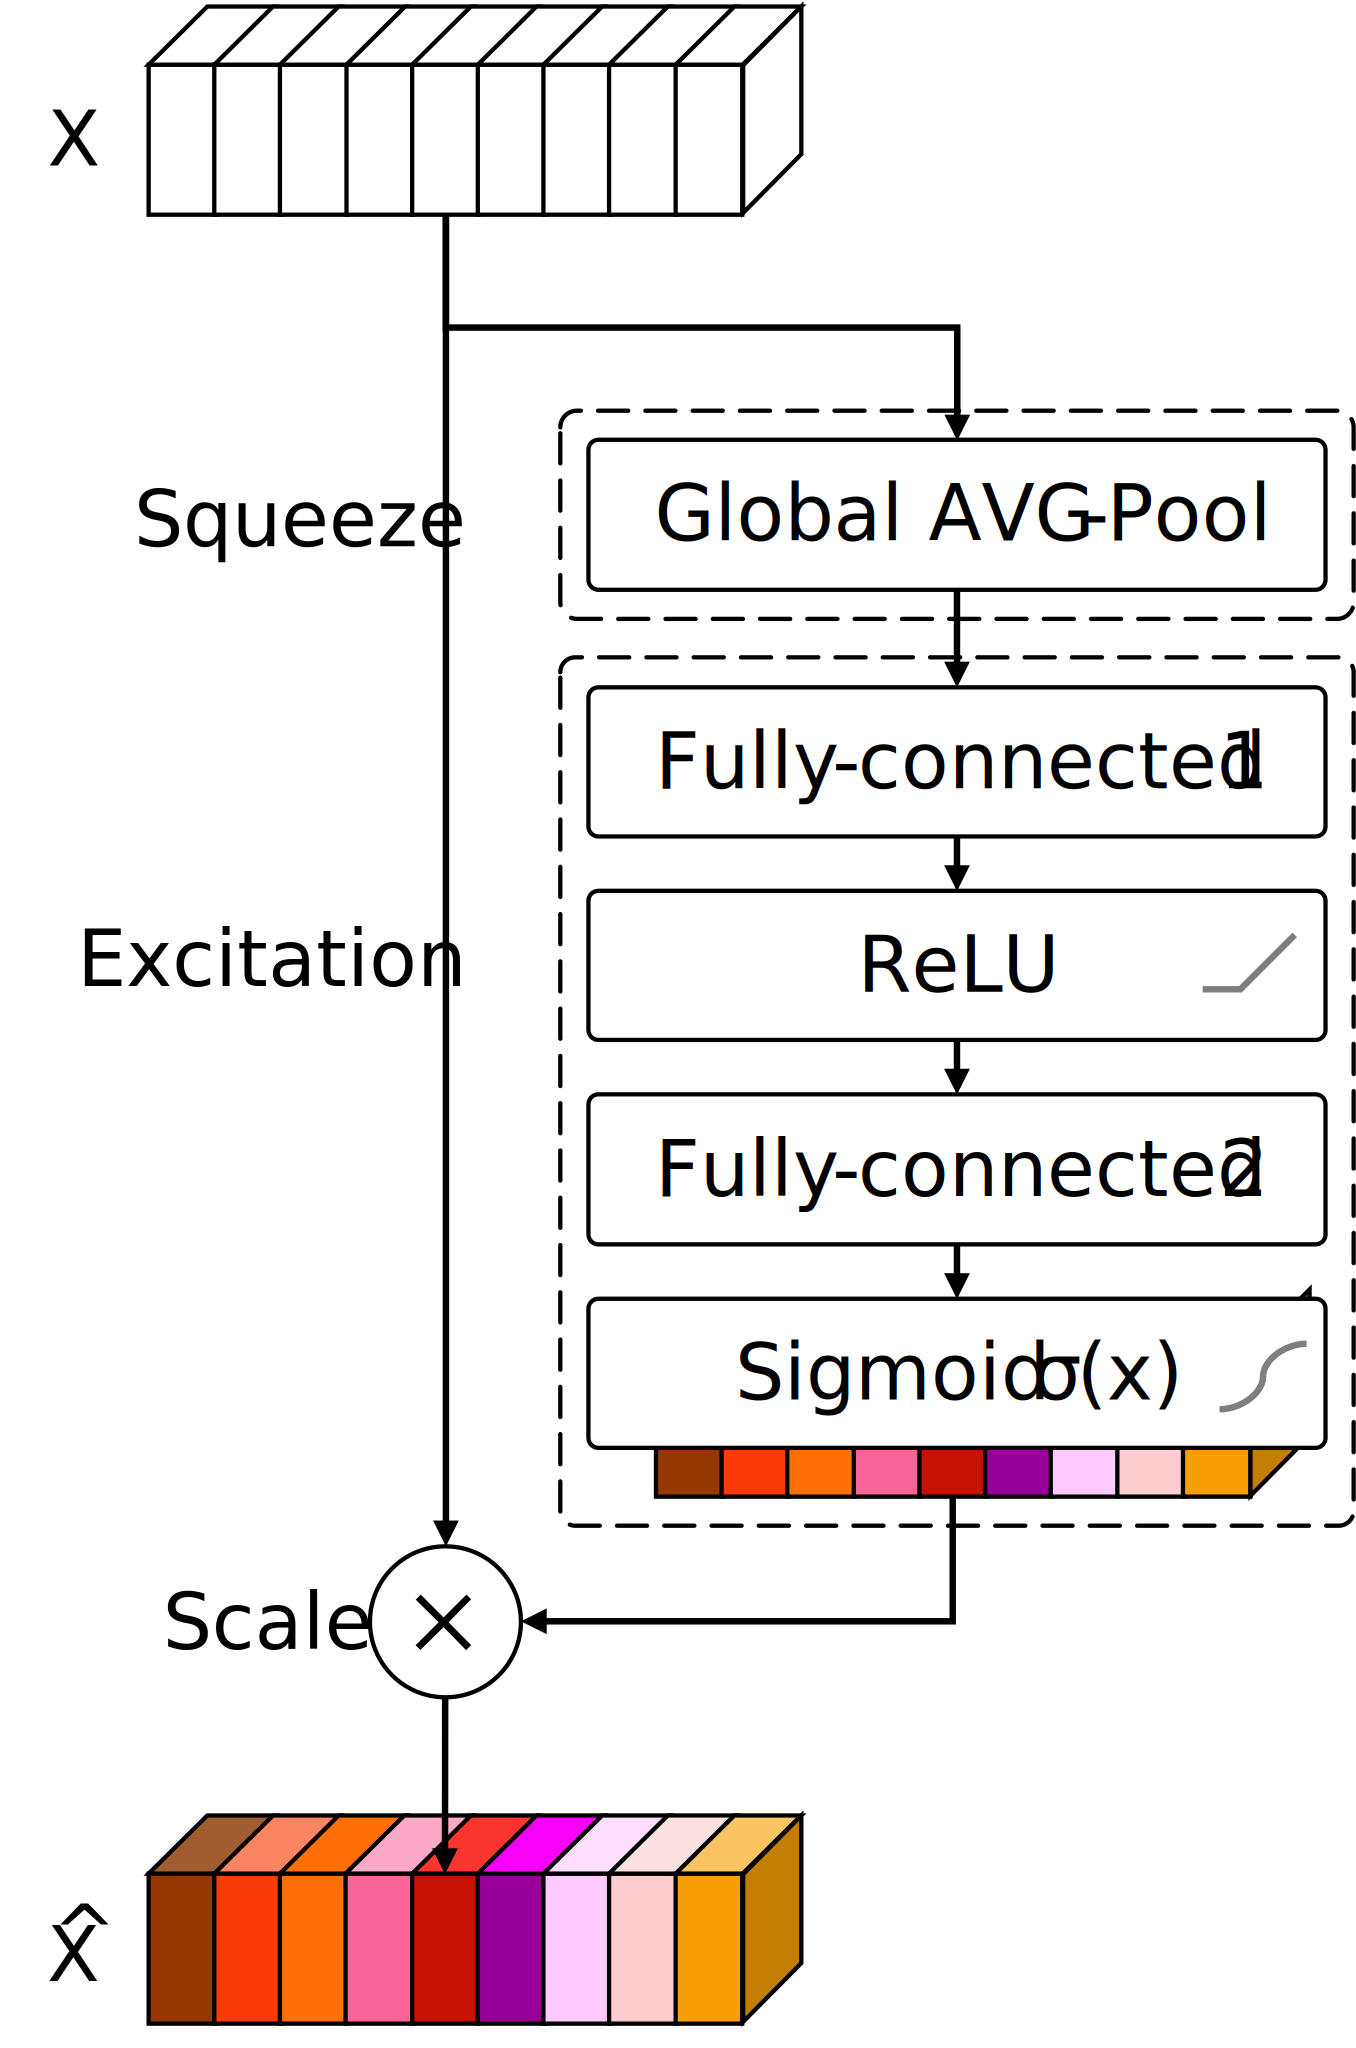
\includegraphics[width=0.3\textwidth]{res/pictures/squeeze-and-excitation-block.pdf}
    % \vspace{-10pt}
    % Das folgende ist ein Trick, um "Abbilgung x.y" in eine
    % eigene Zeile zu packen. Der Text zwischen [ und ] steht
    % im Abbildungsverzeichnis. Der Text darunter wird
    % tats��chlich angezeigt.
    \caption[Squeeze \& Excitation Block]{\unskip}
    Squeeze \& Excitation Block
    \label{fig:squeeze-and-excitation-block}
\end{wrapfigure}

TODO:

\pagebreak

\begin{figure}[!ht]
    \centering
    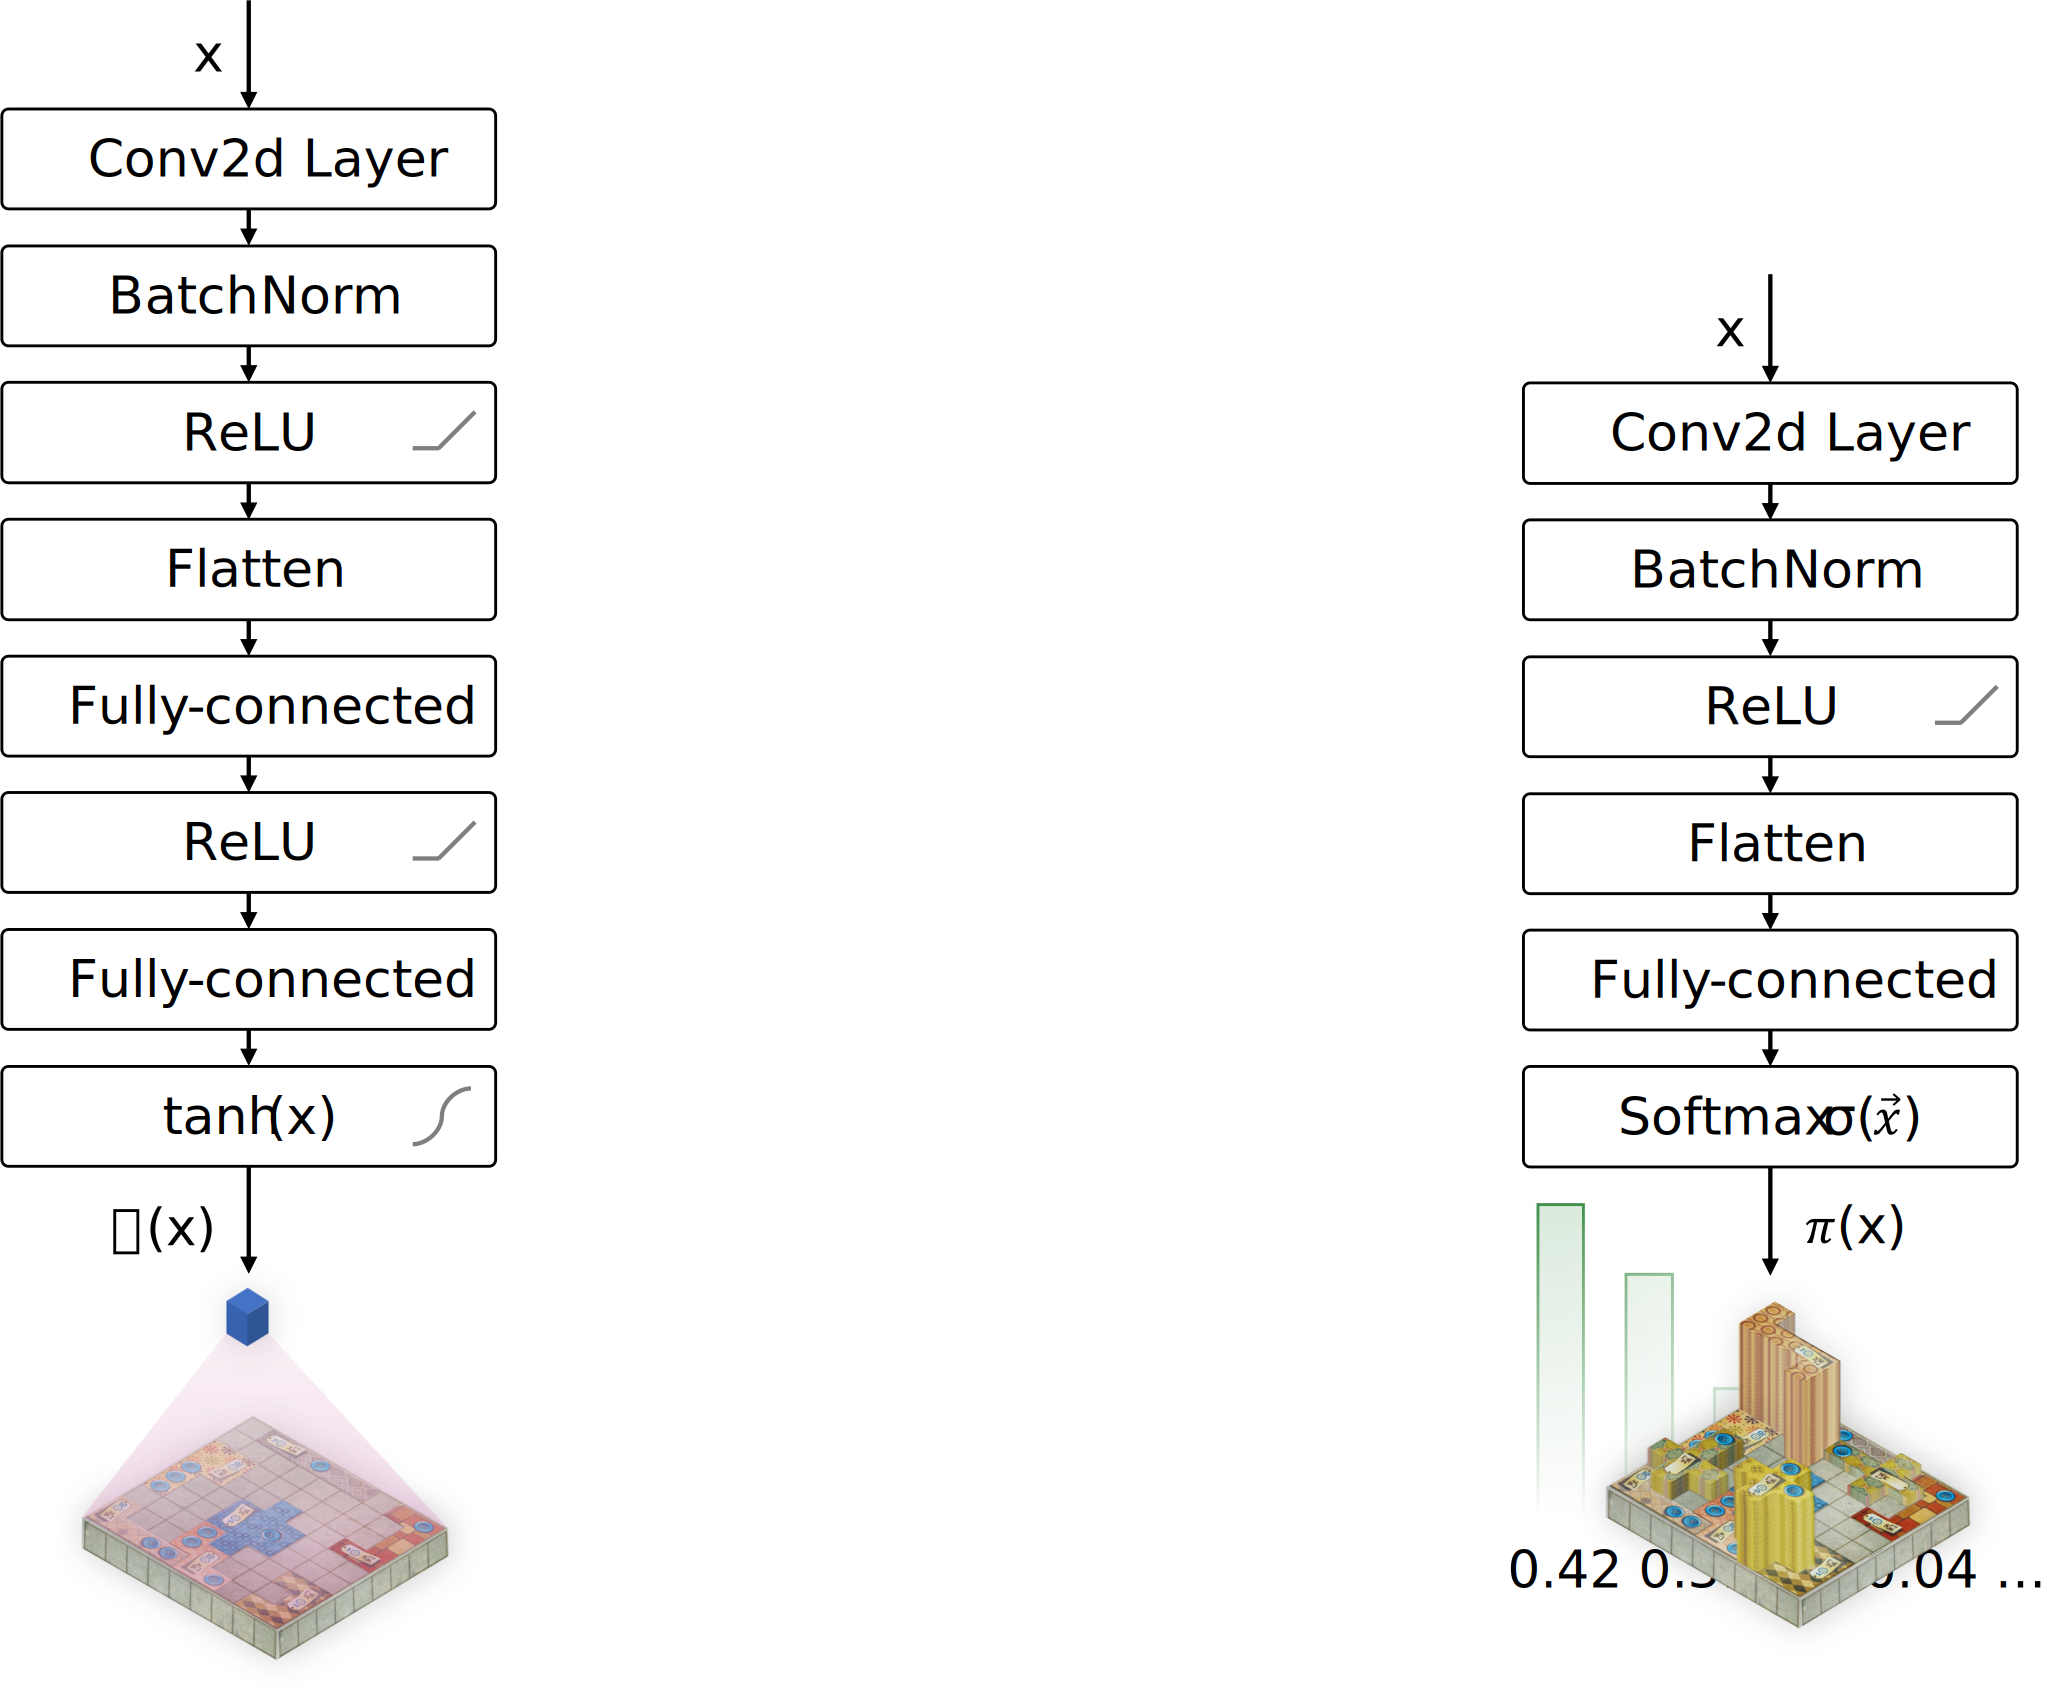
\includegraphics[width=0.7\textwidth]{res/pictures/value-and-policy-head.pdf}
    \\
    \begin{minipage}{.49\textwidth}
        \centering
        \captionof{figure}[Value Head von PatchZero]{\unskip}
        Value Head von PatchZero
        \label{fig:value-head}
    \end{minipage}
    \hfill
    \begin{minipage}{.49\textwidth}
        \centering
        \captionof{figure}[Policy Head von PatchZero]{\unskip}
        Policy Head von PatchZero
        \label{fig:policy-head}
    \end{minipage}
\end{figure}

TODO: